\documentclass{myclass}
\usepackage[polish]{babel}

\numberwithin{equation}{subsection}

\begin{document}
{\footnotesize \tableofcontents}


\section{Wstęp}

Celem tych notatek jest zwięzłe przedstawienie kompletu zagadnień związanych z szeroko pojętym
uczeniem głębokim jako podejściem do Sztucznej Inteligencji (SI). Zaczynamy od minimalnego zbioru
wymaganych tematów z zakresu rachunku prawdopodobieństwa i statystyki matematycznej. Następnie
opisujemy podstawowe metody uczenia maszynowego z probabilistycznego punktu widzenia. W końcu
przechodzimy do zasadniczej części związanej z uczeniem głębokim i sieciami neuronowymi. W każdej
części staramy się przedstawiać opisywane tematy w sposób minimalistyczny, skupiając się głównie na
matematycznej i ideowej, a nie implementacyjnej stronie zagadnień. Liczymy, iż takie podejście
zapewni odpowiednio głębokie zrozumienie tematu, dzięki któremu dalsze studiowanie całej gamy
specyficznych technicznych tematów nie sprawi żadnego problemu.

\subsection{Notacja}

W dalszej części tekstu będziemy stosować przedstawioną tutaj pokrótce notację. Wektory, które
traktujemy jako elementy przestrzeni \(\mathbb{R}^d\) ze standardowo zdefiniowanymi operacjami
dodawania i mnożenia przez skalar będziemy oznaczali wytłuszczonymi małymi literami np. \(\bm{x},
\bm{w}, \bm{\phi}\). Wielkość \(\bm{x}^i\) będzie oznaczać dany element wektora (w tym przypadku
\(i\)--ty element \(\bm{x}\)). Wielkość \(\bm{x}_\mu\) będzie oznaczać pewien (w tym przypadku
\(\mu\)--ty) element pewnego zbioru wektorów. Macierze oraz wielowymiarowe tablice (zwane również
niefortunnie tensorami) będziemy oznaczać wytłuszczonymi wielkimi literami np. \(\bm{X}, \bm{W},
\bm{\Phi}\). Analogicznie jak w przypadku wektorów przez \(\bm{X}^{i_1 i_2 \ldots i_k}\) będziemy
oznaczać \((i_1,i_2,\ldots,i_k)\) element \(k\)--wymiarowej tablicy \(\bm{X}\), natomiast
\(\bm{X}_\mu\) będzie oznaczać \(\mu\)--ty element pewnego zbioru tablic.


\subsection{Uczenie nadzorowane}

Uczenie nadzorowane jest jednym z dwóch podstawowych (pomijając tzw. uczenie ze wzmocnieniem)
paradygmatów w uczeniu maszynowym, którego ogólną ideą jest zdefiniowanie pewnego modelu
odwzorowującego dane wejściowe na wyjściowe predykcje. Zakładamy w nim, iż mamy dostępny zbiór
obserwacji w postaci uporządkowanych par \(\mathcal{X} = \{(\bm{x}_\mu, y_\mu)\}_{\mu=1}^n\), gdzie
\(\bm{x} \in \mathbb{R}^d\) nazywamy wektorem cech a \(y\) jest prawidłową wartością odpowiedzi dla
tych cech. Dwa najbardziej podstawowe przypadki zagadnień tego rodzaju to regresja oraz
klasyfikacja. W przypadku regresji zmienna \(y\) przyjmuje wartości z przedziału liczb
rzeczywistych. W przypadku klasyfikacji zmienna \(y\) przyjmuje wartości ze skończonego zbioru
kategorii, przy czym wartości z tego zbioru nie powinny posiadać naturalnej tj. wynikającej z natury
problemu, relacji porządku; gdy tak nie jest mamy do czynienia z regresją/klasyfikacją porządkową (z
ang. \textit{ordinal regression/classification}).

W jaki sposób tworzymy wspomniany model odwzorowujący \(\bm{x}\) na \(y\)? W dalszych paragrafach
poznamy różne metody, ale najczęściej (nie wchodząc teraz w modelowanie probabilistyczne) modelem
jest pewna rodzina funkcji postaci \(\hat{y}(\bm{x}; \bm{w})\) parametryzowana skończoną liczbą
parametrów, które możemy łącznie zapisać jako pewien wektor \(\bm{w} \in \mathbb{R}^m\). Aby znaleźć
parametry \(\bm{w}\), dzięki którym dla konkretnego zagadnienia model będzie zadowalająco
odwzorowywał cechy na predykcje (innymi słowy aby nauczyć model) wprowadzamy dodatkowo funkcjonał
kosztu (z ang. \textit{loss function}) \(\ell[\hat{y}(\bm{x};\bm{w}), y]\), który kwantyfikuje
odpowiedzi modelu \(\phi\) w stosunku do znanych prawidłowych odpowiedzi \(y\). Trening modelu
polega wówczas na znalezieniu parametrów \(\bm{w}^*\), które minimalizują średnią z wartości funkcji
kosztu dla przykładów w zbiorze treningowym \(\mathcal{X}\)
\begin{equation}
    \bm{w}^* = \arg\min_{\bm{w}} \frac{1}{n}L(\mathcal{X};\bm{w}) = \arg\min_{\bm{w}} \frac{1}{n}\sum_{\mu=1}^n \ell[\hat{y}(\bm{x}_\mu;\bm{w}), y_\mu]\,.
\end{equation}
Zauważmy, że takie podejście ma jedną zasadniczą wadę -- istotnie nie interesuje nas tak naprawdę,
jak model radzi sobie na zbiorze treningowym, tylko jak będzie radził sobie na nowych, niewidzianych
wcześniej danych. Sytuację, w której model bardzo dobrze modeluje dane w zbiorze treningowym, ale
słabo radzi sobie na nowych danych nazywamy przeuczeniem lub nadmiernym dopasowaniem (z ang.
\textit{overfitting}). Sytuację, w której model słabo radzi sobie zarówno na zbiorze treningowym,
jak i na nowych danych nazywamy niedouczeniem lub niedopasowaniem (z ang. \textit{underfitting}).
Występowanie overfittingu i underfittingu jest powiązane z pojemnością (z ang. \textit{capacity})
modelu. Złożony model o dużej pojemności potrafi dopasować się do bardzo skomplikowanych obserwacji,
ale istnieje ryzyko jego przeuczenia (mówimy wówczas o \textit{high variance}). Dla prostego modelu
o małej pojemności istnieje z kolei ryzyko, iż nie ma on wystarczająco ekspresywności (mówimy
wówczas o \textit{high bias}).
 

\subsection{Uczenie nienadzorowane}

W przypadku uczenia nienadzorowanego naszym celem nie jest znalezienie modelu odwzorowującego cechy
na predykcje. Chcemy raczej zrozumieć wewnętrzną strukturę danych. Modele tego rodzaju znajdują
zastosowanie w analizie biznesowej, gdzie pozwalają, chociażby na analizę ważności poszczególnych
wskaźników, czy wizualizację wysoko-wymiarowych danych. Nas będą interesować natomiast szczególnie
generatywne modele nienadzorowane, za pomocą których modelujemy rozkład prawdopodobieństwa danych,
czy to wprost poprzez funkcję gęstości prawdopodobieństwa, czy też jedynie jako model, z którego
możemy próbkować nowe przykłady.


\subsection{Praktyka uczenia maszynowego}

W dalszej części nie będziemy skupiać się na detalach implementacyjnych. W naszej ocenie jednak
dziedzina uczenia maszynowego jest przede wszystkim \enquote{nauką eksperymentalną} dlatego bardzo
ważne jest empiryczne sprawdzenie różnych metod przed wybraniem ostatecznego modelu dla danego
zagadnienia. W tym paragrafie opisujemy standardowe praktyki stosowane przy treningu modeli uczenia
maszynowego (głównie nadzorowanych operujących na danych tabelarycznych).


\subsubsection{Przygotowanie danych}

Kluczem do uzyskania dobrych wyników przy korzystaniu z algorytmów uczenia maszynowego jest
odpowiednie przygotowanie danych (z ang. \textit{preprocessing}). Typowo preprocessing składa się z:

\begin{itemize}
    \item wczytania danych;
    
    \item eksploracji danych oraz wstępnego czyszczenia, w szczególności usunięcia jawnych wartości
    odstających (z ang. \textit{outliers}) oraz cech posiadających zbyt dużo wartości brakujących;

    \item analizy rozkładu zmiennej docelowej oraz ewentualnej transformacji logarytmicznej, która
    poprawia stabilność numeryczną, gdy przewidywane wartości są dużymi dodatnimi liczbami
    rzeczywistymi, zmienia dziedzinę zmiennej objaśnianej z \(\mathbb{R}_+\) na \(\mathbb{R}\) oraz
    dodatkowo jest przykładem transformacji stabilizującej wariancję;
    
    \item \emph{podziału zbioru na część treningową oraz testową};

    \item dokonania skalowania i imputacji brakujących wartości cech (metody \texttt{.fit()}
    wywołujemy jedynie dla zbioru treningowego);

    \item usunięcia silnie skorelowanych cech;

    \item zakodowania wartości kategorycznych za pomocą tzw. \textit{one--hot encoding} pamiętając o
    \textit{dummy variable trap} -- jedną z \(k\) kategorii kodujemy za pomocą wektora
    \textit{one--hot} długości \(n-1\), aby uniknąć zależności liniowej między cechami (opcja
    \texttt{drop="first"} w \texttt{OneHotEncoder} w scikit-learn);

    \item wykonania feature engineering -- dodania wielomianów cech do naszych danych lub
    skonstruowania innych cech (np. cech określających miesiąc, dzień itp.);
\end{itemize}

Podział zbioru na część treningową i testową jest najważniejszym etapem preprocessingu. Zbiór
testowy wydzielamy, aby po wytrenowaniu modelu sprawdzić, jak poradzi on sobie na nowych,
niewidzianych wcześniej danych. Powinniśmy go traktować jako dane, które będziemy w przyszłości
dostawać po wdrożeniu modelu do realnego systemu. Takie dane również będziemy musieli przeskalować,
zakodować itp., ale parametry potrzebne do wykonania tych transformacji możemy wziąć jedynie z
dostępnego wcześniej zbioru treningowego. Wykorzystanie danych testowych w procesie treningu to
\emph{błąd wycieku danych} (z ang. \textit{data leakage}). Skutkuje on niepoprawnym, nadmiernie
optymistycznym oszacowaniem jakości modelu.

\subsubsection{Tuning hiperparametrów i walidacja skrośna}

Praktycznie wszystkie modele uczenia maszynowego mają hiperparametry, często liczne, które w
zauważalny sposób wpływają na wyniki, a szczególnie na underfitting i overfitting. Ich wartości
trzeba dobrać zatem dość dokładnie. Proces doboru hiperparametrów nazywa się tuningiem
hiperparametrów (z ang. \textit{hyperparameter tuning}).

Istnieje na to wiele sposobów. Większość z nich polega na tym, że trenuje się za każdym razem model
z nowym zestawem hiperparametrów i wybiera się ten zestaw, który pozwala uzyskać najlepsze wyniki.
Metody głównie różnią się między sobą sposobem doboru kandydujących zestawów hiperparametrów.
Najprostsze i najpopularniejsze to:
\begin{itemize}
    \item pełne przeszukiwanie (z ang. \textit{grid search}) -- definiujemy możliwe wartości dla
    różnych hiperparametrów, a metoda sprawdza ich wszystkie możliwe kombinacje (czyli siatkę),

    \item losowe przeszukiwanie (z ang. \textit{randomized search}) -- definiujemy możliwe wartości
    jak w pełnym przeszukiwaniu, ale sprawdzamy tylko ograniczoną liczbę losowo wybranych
    kombinacji.
\end{itemize}

Jak ocenić, jak dobry jest jakiś zestaw hiperparametrów? Nie możemy sprawdzić tego na zbiorze
treningowym -- wyniki byłyby zbyt optymistyczne. Nie możemy wykorzystać zbioru testowego --
mielibyśmy wyciek danych, bo wybieralibyśmy model explicite pod nasz zbiór testowy. Trzeba zatem
osobnego zbioru, na którym będziemy na bieżąco sprawdzać jakość modeli dla różnych hiperparametrów.
Jest to zbiór walidacyjny (z ang. \textit{validation set}). Zbiór taki wycina się ze zbioru
treningowego.

Jednorazowy podział zbioru na części nazywa się \textit{split validation} lub \textit{holdout}.
Używamy go, gdy mamy sporo danych, i 10-20\% zbioru jako dane walidacyjne czy testowe to dość dużo,
żeby mieć przyzwoite oszacowanie. Zbyt mały zbiór walidacyjny czy testowy da nam mało wiarygodne
wyniki -- nie da się nawet powiedzieć, czy zbyt pesymistyczne, czy optymistyczne. W praktyce
niestety często mamy mało danych. Trzeba zatem jakiejś magicznej metody, która stworzy nam więcej
zbiorów walidacyjnych z tej samej ilości danych. Taką metodą jest walidacja skrośna (z ang.
\textit{cross validation}, CV). Polega na tym, że dzielimy zbiór treningowy na \(K\) równych
podzbiorów, tzw. foldów. Każdy podzbiór po kolei staje się zbiorem walidacyjnym, a pozostałe łączymy
w zbiór treningowy. Trenujemy zatem \(K\) modeli dla tego samego zestawu hiperparametrów i każdy
testujemy na zbiorze walidacyjnym. Mamy \(K\) wyników dla zbiorów walidacyjnych, które możemy
uśrednić (i ewentualnie obliczyć odchylenie standardowe). Takie wyniki są znacznie bardziej
wiarygodne.



\section{Rachunek prawdopodobieństwa i statystyka}


\subsection{Przestrzeń probabilistyczna}

Pojęciem pierwotnym w rachunku prawdopodobieństwa jest pojęcie \emph{przestrzeni zdarzeń
elementarnych}, którą oznaczamy \(\Omega\). W przypadku doświadczeń losowych przestrzeń zdarzeń
elementarnych jest zbiorem wszystkich niepodzielnych wyników obserwacji.

\begin{definition}[Rodziny zdarzeń]

Niech \(\Omega\) będzie przestrzenią zdarzeń elementarnych. Rodziną zdarzeń nazwiemy rodzinę zbiorów
\(\mathcal{F}\) taką, że
\begin{enumerate}
    
    \item \(\Omega \in \mathcal{F}\).
    
    \item Jeśli \(A \in \mathcal{F}\) to \(\Omega \setminus A \in \mathcal{F}\).
    
    \item Jeśli \(A_1,A_2,\ldots \in \mathcal{F}\) to \(\bigcup_{i=1}^\infty A_i \in \mathcal{F}\).

\end{enumerate}

Rodzinę zdarzeń \(\mathcal{F}\) nazywamy \(\sigma\)--ciałem zdarzeń losowych.

\end{definition}

\begin{definition}[Zdarzenia losowego]
    Zdarzeniem losowym nazywamy dowolny zbiór należący do rodziny zdarzeń \(\mathcal{F}\). W
    szczególności \(\Omega\) nazwiemy zdarzeniem pewnym, a \(\emptyset\) -- zdarzeniem niemożliwym.
\end{definition}

\begin{definition}[Rozkładu prawdopodobieństwa]
Niech dana będzie przestrzeń zdarzeń elementarnych \(\Omega\) i rodzina zdarzeń \(\mathcal{F}\).
Rozkładem prawdopodobieństwa nazwiemy funkcję \(\Pr: \mathcal{F} \mapsto [0;1]\) spełniającą
\begin{enumerate}
    
    \item Dla każdego \(A \in \mathcal{F}\) zachodzi \(\Pr(A) \geq 0\).
    
    \item \(\Pr(\Omega) = 1\).
    
    \item Dla każdego ciągu zdarzeń parami rozłącznych \(A_1,A_2,\ldots\), \(\forall i \neq j : A_i
    \cap A_j = \emptyset\) zachodzi
    \begin{equation*}
        \Pr\left(\bigcup_{i=1}^\infty A_i\right) = \sum_{i=1}^\infty \Pr(A_i)\,.
    \end{equation*}

\end{enumerate}
\end{definition}

\begin{theorem}
Niech \(\Pr\) będzie rozkładem prawdopodobieństwa w rodzinie zdarzeń \(\mathcal{F}\), wówczas

\begin{enumerate}
    
    \item \(\Pr(\emptyset) = 1\).
    
    \item (Addytywność) Dla dowolnych zdarzeń \(A_1,\ldots,A_n\) parami rozłącznych zachodzi
    \begin{equation*}
        \Pr\left(\bigcup_{i=1}^n A_i\right) = \sum_{i=1}^n \Pr(A_i)\,.
    \end{equation*}

    \item Dla dowolnego zdarzenia \(A\) zachodzi
    \begin{equation*}
        \Pr(A') = 1 - \Pr(A)\,.
    \end{equation*}

    \item Dla dowolnych zdarzeń \(A, B\) zachodzi
    \begin{equation*}
        \Pr(A \cup B) = \Pr(A) + \Pr(B) - \Pr(A \cap B)\,.
    \end{equation*}

    \item Jeśli \(A \subset B\) to \(\Pr(A) \leq \Pr(B)\).

    \item Dla każdego zdarzenia \(A\) zachodzi \(\Pr(A) \leq 1\).

\end{enumerate}
\end{theorem}

\begin{definition}[Przestrzeni probabilistycznej]
Przestrzenią probabilistyczną nazywamy uporządkowaną trójkę \((\Omega, \mathcal{F}, \Pr)\), gdzie
\(\Omega\) jest przestrzenią zdarzeń elementarnych, \(\mathcal{F}\) -- rodziną zdarzeń określoną na
\(\Omega\), a \(\Pr\) -- rozkładem prawdopodobieństwa w \(\mathcal{F}\).
\end{definition}


\subsection{Prawdopodobieństwo warunkowe i niezależność zdarzeń}

\begin{definition}[Prawdopodobieństwa warunkowego]
Jeśli \(\Pr(B) > 0\) to prawdopodobieństwem \(\Pr(A \mid B)\) zdarzenia \(A\) pod warunkiem
zdarzenia \(B\) nazywamy iloraz prawdopodobieństw

\begin{equation*}
    \Pr(A \mid B) := \frac{\Pr(A \cap B)}{ \Pr(B)}\,.
\end{equation*}
\end{definition}

Można pokazać, iż prawdopodobieństwo warunkowe jako funkcja zdarzenia \(A\) przy ustalonym zdarzeniu
\(B\) spełnia wszystkie aksjomaty rozkładu prawdopodobieństwa.

\begin{theorem}[O wielokrotnym warunkowaniu]
Dla dowolnych zdarzeń \(A_1,\ldots,A_n\) takich, że \(\Pr(A_1,\ldots,A_n) > 0\) zachodzi
\begin{equation*}
    \begin{split}
        &\Pr(A_1,\ldots,A_n) =\\
        &\Pr(A_n \mid A_{n-1},\ldots,A_1) \ldots \Pr(A_2 \mid A_1) \Pr(A_1)\,,
    \end{split}
\end{equation*}
gdzie dla uproszczenia zapisu używamy \(\Pr(A,B)\) w znaczeniu \(\Pr(A \cap B)\).
\end{theorem}

\begin{definition}[Niezależności pary zdarzeń]
Zdarzenia \(A, B\) nazwiemy niezależnymi jeśli
\begin{equation*}
    \Pr(A, B) = \Pr(A) \Pr(B)\,.
\end{equation*}
\end{definition}

Zauważmy, iż w przypadku \(\Pr(B) > 0\) powyższa definicja jest równoważna bardziej intuicyjnej
wynikającej z definicji prawdopodobieństwa warunkowego, mianowicie zdarzenia \(A,B\) nazywamy
niezależnymi jeśli \(\Pr(A \mid B) = \Pr(A)\).

\begin{definition}[Niezależności zdarzeń]
Zdarzenia \(A_1,\ldots,A_n\) nazwiemy niezależnymi, jeśli dla dowolnych wskaźników
\(k_1,\ldots,k_s\), gdzie \(1 \leq k_1 < \ldots < k_s \leq n\) zachodzi
\begin{equation*}
    \Pr(A_{k_1},\ldots,A_{k_s}) = \Pr(A_{k_1}) \ldots \Pr(A_{k_s})\,.
\end{equation*}
\end{definition}

\begin{theorem}[O łącznym prawdopodobieństwie niezależnych zdarzeń]
Jeśli zdarzenia \(A_1,\ldots,A_n\) są niezależne to
\begin{equation*}
    \Pr(A_1,\ldots,A_n) = \Pr(A_1) \ldots \Pr(A_n)\,.
\end{equation*}
\end{theorem}

\begin{definition}[Warunkowej niezależności pary zdarzeń]
Zdarzenia \(A,B\) są warunkowo niezależne względem \(C\) jeśli
\begin{equation*}
    \Pr(A,B \mid C) = \Pr(A \mid C) \Pr(B \mid C)\,.
\end{equation*}
\end{definition}

\begin{definition}[Warunkowej niezależności zdarzeń]
Zdarzenia \(A_1,\ldots,A_n\) są warunkowo niezależne względem \(B\) jeśli dla dowolnych wskaźników
\(k_1,\ldots,k_s\), gdzie \(1 \leq k_1 < \ldots < k_s \leq n\) zachodzi
\begin{equation*}
    \Pr(A_{k_1},\ldots,A_{k_s} \mid B) = \Pr(A_{k_1} \mid B) \ldots \Pr(A_{k_s} \mid B)\,.
\end{equation*}
\end{definition}

\begin{theorem}
Jeśli zdarzenia \(A_1,\ldots,A_n\) są warunkowo niezależne względem \(B\) to
\begin{equation*}
    \Pr(A_1,\ldots,A_n \mid B) = \Pr(A_1 \mid B) \ldots \Pr(A_n \mid B)\,.
\end{equation*}
\end{theorem}


\subsection{Prawdopodobieństwo całkowite i wzór Bayesa}

\begin{definition}[Układu zupełnego zdarzeń]
Jeśli zdarzenia \(A_1,A_2\ldots,\) są parami rozłączne oraz \(\bigcup_{i=1}^\infty A_i = \Omega\) to
zbiór zdarzeń \(\{A_i\}\) nazywamy układem zupełnym.
    
\end{definition}

\begin{theorem}[O prawdopodobieństwie całkowitym]
Jeśli zdarzenia \(A_i\) (gdzie \(i\) przebiega przeliczalny zbiór wartości) tworzą układ zupełny
zdarzeń oraz \(\Pr(A_i) > 0\) dla każdego \(i\), to dla dowolnego zdarzenia \(B\) zachodzi
\begin{equation*}
    \Pr(B) = \sum_{i} \Pr(B \mid A_i) \Pr(A_i)\,.
\end{equation*}
\end{theorem}

\begin{theorem}[Bayesa]
Jeśli zdarzenia \(A_i\) spełniają założenia tw. o prawdopodobieństwie całkowitym oraz \(\Pr(B) >
0\), to dla każdego zdarzenia \(A_j\) z rozpatrywanego układu zdarzeń zachodzi
\begin{equation*}
    \Pr(A_j \mid B) = \frac{\Pr(B \mid A_j) \Pr(A_j)}{\Pr(B)} = \frac{\Pr(B \mid A_j) \Pr(A_j)}{\sum_{i} \Pr(B \mid A_i) \Pr(A_i)}\,.
\end{equation*}
Prawdopodobieństwa \(\Pr(A_j)\) nazywamy prawdopodobieństwami \emph{a priori}, a \(\Pr(A_j \mid B)\)
-- \emph{a posteriori}. Prawdopodobieństwo \(\Pr(B \mid A_j)\) nazywamy \emph{wiarygodnością}.   
\end{theorem}


\subsection{Zmienne losowe}

\begin{definition}[Zmiennej losowej]
Niech \((\Omega, \mathcal{F}, \Pr)\) będzie przestrzenią probabilistyczną. Niech dany będzie również
drugi zbiór \(\mathcal{X}\), w którym wyróżniamy \(\sigma\)--ciało \(\mathcal{F}_\mathcal{X}\).
Zmienną losową \(X\) nazywamy odwzorowanie
\begin{equation*}
    X: \Omega \mapsto \mathcal{X}
\end{equation*}
takie, że dla każdego \(A \in \mathcal{F}_\mathcal{X}\) zachodzi warunek
\begin{equation*}
    \{\omega \in \Omega : X(\omega) \in A \} \in \mathcal{F}\,.
\end{equation*}
\end{definition}

W szczególności jeśli \(\mathcal{X} = \mathbb{R}\) to zmienną losową \(X\) nazywamy \emph{zmienną
losową rzeczywistą}, natomiast jeśli \(\mathcal{X} = \mathbb{R}^n\) to zmienną losową \(\bm{X}\)
nazywamy \emph{zmienną losową \(n\)--wymiarową}.

\begin{definition}[Rozkładu prawdopodobieństwa zmiennej losowej]
Niech \(X: \Omega \mapsto \mathcal{X}\) będzie zmienną losową. Funkcję \(\Pr_X:
\mathcal{F}_\mathcal{X}\mapsto [0;1]\) określoną jako
\begin{equation*}
    {\Pr_{X}} (A) = \Pr(\{\omega \in \Omega : X(\omega) \in A\})
\end{equation*}
nazywamy rozkładem prawdopodobieństwa zmiennej losowej \(X\).
\end{definition}

W dalszym ciągu będziemy stosować notację uproszczoną pomijając indeks dolny \(X\) tj.
\begin{equation*}
    \Pr(X \in A) := \Pr(\{\omega \in \Omega : X(\omega) \in A\})\,.
\end{equation*}

Znajomość rozkładu zmiennej losowej \(X\) pozwala badać własności tej zmiennej bez znajomości
przestrzeni probabilistycznej \((\Omega, \mathcal{F}, \Pr)\), na której owa zmienna jest określona.
Możemy mianowicie zawsze rozpatrywać tę zmienną jako określoną na przestrzeni probabilistycznej
\((\mathcal{X}, \mathcal{F}_\mathcal{X}, \Pr_X)\).

\begin{definition}[Dystrybuanty zmiennej losowej rzeczywistej]
Niech \(X: \Omega \mapsto \mathbb{R}\) będzie zmienną losową rzeczywistą. Dystrybuantą zmiennej
losowej \(X\) nazywamy funkcję \(F: \mathbb{R} \mapsto [0;1]\) zdefiniowaną jako
\begin{equation*}
    F(x) = \Pr(X \leq x)\,.
\end{equation*}
\end{definition}

\begin{theorem}[Własności dystrybuanty zmiennej rzeczywistej]
Niech \(F\) będzie dystrybuantą zmiennej losowej rzeczywistej \(X\), wówczas
\begin{enumerate}
    
    \item Jeśli \(a < b\) to \(F(b) - F(a) = \Pr( a < X \leq b )\).
    
    \item Funkcja \(F\) jest niemalejąca.

    \item \(\lim_{x \to -\infty} F(x) = 0\) oraz \(\lim_{x \to +\infty} F(x) = 1\).

    \item \(F\) jest prawostronnie ciągła.

    \item \(F\) jest ciągła w \(x_0\) wtedy i tylko wtedy, gdy \(\Pr(X = x_0) = 0\).

\end{enumerate}
\end{theorem}

\begin{definition}[Rozkładu dyskretnego zmiennej losowej rzeczywistej]
Mówimy, że zmienna losowa rzeczywista \(X\) ma rozkład dyskretny jeśli istnieje skończony lub
przeliczalny zbiór \(\mathcal{S} \subset \mathbb{R}\) taki, że
\begin{equation*}
    \Pr( X \in \mathcal{S} ) = 1\,.
\end{equation*}
Dla takiej zmiennej określa się funkcję prawdopodobieństwa (z ang. \textit{probability mass
function, pmf})
\begin{equation*}
    p(x) = \Pr(X = x)\,,\quad x \in \mathcal{S}\,.
\end{equation*}
\end{definition}

Zauważmy, że jeśli zmienna \(X\) ma rozkład dyskretny to zbiór \(\mathcal{S}\) ma postać
\(\{x_1,\ldots,x_k\}\) dla pewnych \(x_i \in \mathbb{R}\).

\begin{definition}[Rozkładu ciągłego zmiennej losowej rzeczywistej]
Mówimy, że zmienna losowa rzeczywista \(X\) ma rozkład ciągły jeśli istnieje funkcja \(p: \mathbb{R}
\mapsto [0; +\infty)\) taka, że dla dowolnego przedziału \((a;b)\) zachodzi
\begin{equation*}
    \Pr(X \in (a;b)) = \int\limits_a^b p(x) \dd{x}\,.
\end{equation*}
Funkcję \(p\) nazywamy gęstością rozkładu prawdopodobieństwa (z ang. \textit{probability density
function, pdf}).
\end{definition}

Jeśli \(X\) jest zmienną losową rzeczywistą o rozkładzie ciągłym to wartość dystrybuanty jest dana
przez
\begin{equation}
    F(x) = \int\limits_{-\infty}^x p(x') \dd{x'}\,.
\end{equation}
W szczególności dystrybuanta \(F\) jest ciągła oraz dla każdego \(x\) zachodzi \(\Pr(X = x) = 0\).

\begin{definition}[Wartości oczekiwanej zmiennej losowej rzeczywistej]
Wartością oczekiwaną zmiennej losowej rzeczywistej \(X\) nazywamy liczbę \(m\) określoną wzorem
\begin{equation*}
    m = \int\limits_{-\infty}^{+\infty} x p(x) \dd{x}
\end{equation*}
dla rozkładu ciągłego oraz
\begin{equation*}
    m = \sum_{x \in \mathcal{S}} x p(x)
\end{equation*}
dla rozkładu dyskretnego. Stosujemy dodatkowo oznaczenie \(\mathbb{E}[X] := m\).
\end{definition}

\begin{definition}[Wariancji zmiennej losowej rzeczywistej]
Wariancją zmiennej losowej rzeczywistej \(X\) nazywamy liczbę \(\sigma\) określoną wzorem
\begin{equation*}
    \sigma^2 = \mathbb{E}[(X - m)^2]\,,
\end{equation*} 
gdzie \(m = \mathbb{E}[X]\). Stosujemy dodatkowo oznaczenie \(\mathbb{V}[X] := \sigma^2\).
\emph{Odchyleniem standardowym} zmiennej losowej \(X\) nazywamy pierwiastek jej wariancji
\begin{equation*}
    \sigma = \sqrt{\mathbb{V}[X]}\,.
\end{equation*} 
\end{definition}

\begin{theorem}[Własności wariancji]
Niech \(X\) będzie zmienną losową rzeczywistą, wówczas
\begin{enumerate}
    
    \item \(\mathbb{V}[X] = \mathbb{E}[X^2] - (\mathbb{E}[X])^2\)\,.

    \item Jeśli zmienna \(X\) ma skończoną wariancję, to dla dowolnych \(a,b \in \mathbb{R}\)
    zachodzi
    \begin{equation*}
        \mathbb{V}[aX + b] = a^2 \mathbb{V}[X]\,.
    \end{equation*}

    \item \(\mathbb{V}[X] = 0\) wtedy i tylko wtedy, gdy istnieje \(x_0 \in \mathbb{R}\) takie, że
    \begin{equation*}
        \Pr(X \neq x_0) = 0\,.
    \end{equation*}

\end{enumerate}
\end{theorem}

\begin{definition}[Zmiennej standaryzowanej]
Zmienną losową o wartości oczekiwanej 0 i wariancji 1 nazywamy zmienną standaryzowaną. Jeśli \(X\)
jest dowolną zmienną o niezerowej wariancji, to
\begin{equation*}
    Z := \frac{X - m}{\sigma}
\end{equation*}
jest zmienną standaryzowaną, ponieważ
\begin{equation*}
    \mathbb{E}[Z] = \frac{1}{\sigma}\mathbb{E}[X - m] = \frac{1}{\sigma}(m - m) = 0
\end{equation*}
oraz
\begin{equation*}
    \mathbb{V}[Z] = \frac{1}{\sigma^2} \mathbb{V}[X] = \frac{\sigma^2}{\sigma^2} = 1\,.
\end{equation*}
\end{definition}

\begin{theorem}[Nierówność Czebyszewa]
Jeśli zmienna losowa \(X\) ma skończoną wartość średnią \(m\) i wariancję \(\sigma^2\), to dla
dowolnego \(\epsilon > 0\) zachodzi
\begin{equation*}
    \Pr(|X - m| \geq \epsilon\sigma) \leq \frac{1}{\epsilon^2}\,.
\end{equation*}
\end{theorem}

\begin{definition}[Kwantyla]
Kwantylem rzędu \(p \in (0;1)\) zmiennej losowej o dystrybuancie \(F\) nazywamy dowolną liczbę
\(q_p\) taką, że
\begin{equation*}
    F(q_p^-) \leq p \leq F(q_p)\,.
\end{equation*}
Kwantyl rzędu 0.5 nazywamy \emph{medianą}, kwantyl rzędu 0.25 -- \emph{dolnym kwartylem}, a kwantyl
rzędu 0.75 -- \emph{górnym kwartylem}. Jeśli \(X\) ma rozkład ciągły, to kwantylem rzędu \(p\) jest
dowolne rozwiązanie równania
\begin{equation*}
    F(q_p) = p\,.
\end{equation*}
\end{definition}

\begin{definition}[Mody]
Modą zmiennej losowej o rozkładzie dyskretnym nazywa się dowolne maksimum funkcji prawdopodobieństwa
tego rozkładu.

Modą zmiennej losowej o rozkładzie ciągłym nazywa się dowolne maksimum lokalne gęstości tego
rozkładu.
\end{definition}


\subsection{Ważne rozkłady jednowymiarowe}

\begin{definition}[Rozkładu jednopunktowego]
Jeśli \(X\) jest zmienną losową rzeczywistą o rozkładzie dyskretnym i \(\mathcal{S} = \{x_0\}\), to
mówimy, że \(X\) ma rozkład jednopunktowy, wówczas
\begin{equation*}
    m = x_0,\quad \sigma^2 = 0\,.
\end{equation*}
\end{definition}

\begin{definition}[Rozkładu dwupunktowego]
Jeśli \(X\) jest zmienną losową rzeczywistą o rozkładzie dyskretnym i \(\mathcal{S} = \{x_1, x_2\}\)
oraz \(p(x_1) = p\), to mówimy, że \(X\) ma rozkład dwupunktowy z parametrem \(p\), wówczas
\begin{equation*}
    m = x_1 p + x_2 (1 - p)\,,\quad \sigma^2 = p (1 - p) (x_1 - x_2)^2\,.
\end{equation*}
Jeśli \(x_1 = 1\) i \(x_2 = 0\) to taki rozkład dwupunktowy nazywamy \emph{rozkładem
zero--jedynkowym} (lub rozkładem Bernoulliego) i oznaczamy jako \(X \sim \mathrm{Ber}(p)\).
\end{definition}

\begin{definition}[Schematu dwumianowego]
Rozważmy doświadczenie losowe o dwu możliwych wynikach: sukces osiągamy z prawdopodobieństwem \(p\),
porażkę z prawdopodobieństwem \(1-p\). Doświadczenie tego rodzaju nazywamy \emph{próbą
Bernoulliego}. Doświadczenie takie jest modelowane zmienną losową o rozkładzie dwupunktowym z
parametrem \(p\). Schematem dwumianowym (lub schematem Bernoulliego) nazywamy doświadczenie
polegające na \(n\)--krotnym powtórzeniu próby Bernoulliego, przy założeniu, iż poszczególne próby
są od siebie niezależne.
\end{definition}

\begin{definition}[Rozkładu dwumianowego]
Niech \(X\) będzie zmienną losową taką, że \(X\) jest liczbą sukcesów w schemacie dwumianowym
długości \(n\) z prawdopodobieństwem sukcesu w każdej próbie równym \(p\). Wówczas
\begin{equation*}
    \Pr(X = k) = {n \choose k} p^k (1 - p)^{n-k}\,.
\end{equation*}
Rozkład prawdopodobieństwa określony powyższym wzorem nazywam się rozkładem dwumianowym o
parametrach \(n,p\). Jeśli zmienna \(X\) ma rozkład dwumianowy to stosujemy notację \(X \sim
\mathrm{Bin}(n,p)\). Jeśli \(X \sim \mathrm{Bin}(n,p)\) to
\begin{equation*}
    m = np\,,\quad \sigma^2 = np(1-p)\,.
\end{equation*}
\end{definition}

\begin{definition}[Rozkładu geometrycznego]
Mówimy, że zmienna losowa \(X\) ma rozkład geometryczny z parametrem \(p \in (0;1)\), tj. \(X \sim
\mathrm{Geo}(p)\), jeśli \(\mathcal{S} = \mathbb{N} \setminus \{0\}\), a funkcja prawdopodobieństwa
ma postać
\begin{equation*}
    p(x) = (1-p)^{x-1}p\,.
\end{equation*}
Zmienna \(X\) opisuje czas oczekiwania na pierwszy sukces w schemacie dwumianowym o nieskończonej
długości. Jeśli \(X \sim \mathrm{Geo}(p)\), to
\begin{equation*}
    m = p^{-1}\,,\quad \sigma^2 = \frac{1 - p}{p^2}\,.
\end{equation*}
\end{definition}

\begin{definition}[Rozkładu Poissona]
Jeśli zmienna \(X\) o wartościach w \(\mathbb{N}\) opisuje liczbę wystąpień pewnego powtarzalnego
zdarzenia w przedziale czasowym \([0;t]\), przy czym spełnione są następujące założenia:
\begin{itemize}

    \item powtórzenia zdarzenia występują niezależnie od siebie;
    
    \item \enquote{intensywność} wystąpień \(r\) jest stała;

    \item w danej chwili (rozumianej jako odpowiednio mały przedział) może zajść co najwyżej jedno
    zdarzenie

\end{itemize}

to zmienna ta ma rozkład Poissona z parametrem \(\lambda = rt\), tj. \(X \sim
\mathrm{Pos}(\lambda)\). Jeśli \(X \sim \mathrm{Pos}(\lambda)\), to
\begin{equation*}
    \Pr(X = k) = \frac{\e^{-\lambda} \lambda^k}{k!}\,.
\end{equation*}
Ponadto
\begin{equation*}
    m = \lambda\,,\quad \sigma^2 = \lambda\,.
\end{equation*}
\end{definition}

\begin{theorem}[Poissona]
Niech \((X_n)\) będzie ciągiem zmiennych losowych takich, że \(X_n \sim \mathrm{Bin}(n, p_n)\),
gdzie \((p_n)\) jest ciągiem takim, że
\begin{equation*}
    \lim_{n \to \infty} n p_n = \lambda
\end{equation*}
dla pewnej liczby \(\lambda > 0\). Wówczas
\begin{equation*}
    \lim_{n \to \infty} \Pr(X_n = k) = \frac{\e^{-\lambda} \lambda^k}{k!}\,.
\end{equation*}
\end{theorem}

\begin{definition}[Rozkładu jednostajnego]
Mówimy, że zmienna \(X\) o rozkładzie ciągłym ma rozkład jednostajny na przedziale \([a;b]\) tzn.
\(X \sim \mathcal{U}(a,b)\) jeśli jej gęstość wyraża się wzorem
\begin{equation*}
    p(x) = \begin{cases}
        \frac{1}{b - a}\,, &x\in[a;b]\\
        0\,,&x\notin[a;b]
    \end{cases}\quad.
\end{equation*}
Jeśli \(X \sim \mathcal{U}(a,b)\), to
\begin{equation*}
    m = \frac{a+b}{2}\,,\quad \sigma^2 = \frac{(b-a)^2}{12}\,.
\end{equation*}
\end{definition}

\begin{definition}[Rozkładu wykładniczego]
Niech \(T\) będzie zmienną modelującą czas oczekiwania na pierwsze zdarzenie w ciągu zdarzeń takim,
że czas wystąpienia każdego z nich w przedziale \([0;t]\) jest opisany przez zmienną \(X \sim
\mathrm{Pos}(\lambda t)\). wtedy
\begin{equation*}
    \Pr(T > t) = \Pr(X = 0) = \e^{-\lambda t}
\end{equation*}
oraz
\begin{equation*}
    \Pr(T > 0) = 1\,.
\end{equation*}
Mówimy wtedy, że \(T\) ma rozkład wykładniczy z parametrem \(\lambda\), tzn. \(T \sim
\mathrm{Exp}(\lambda)\). Gęstość rozkładu wykładniczego ma postać
\begin{equation*}
    p(t) = \begin{cases}
        0\,,&t \leq 0\\
        \lambda \e^{-\lambda t}\,,&t > 0
    \end{cases}\quad.
\end{equation*}
Jeśli \(T \sim \mathrm{Exp}(\lambda)\), to
\begin{equation*}
    m = \lambda^{-1}\,,\quad \sigma^2 = \lambda^{-2}\,.
\end{equation*}
\end{definition}

\begin{definition}[Rozkładu normalnego]
Mówimy, że zmienna losowa \(X\) o gęstości \(\phi(x;\mu,\sigma^2)\) ma rozkład normalny z
parametrami \(\mu \in \mathbb{R} , \sigma^2 \in [0;+\infty)\), tzn. \(X \sim
\mathcal{N}(\mu,\sigma^2)\), jeśli    
\begin{equation*}
    \phi(x; \mu, \sigma^2) = \frac{1}{\sqrt{2 \pi \sigma^2}} \exp\left(-\frac{(x-\mu)^2}{2\sigma^2}\right)\,.
\end{equation*}
Jeśli \(X \sim \mathcal{N}(\mu,\sigma^2)\), to
\begin{equation*}
    m = \mu\,,\quad \mathbb{V}[X] = \sigma^2\,.
\end{equation*}
\end{definition}

Jeśli \(X \sim \mathcal{N}(\mu,\sigma^2)\), to
\begin{equation}
    \begin{split}        
        &\Pr(|X - m| > 2\sigma) \approx 0.0455003\,,\\
        &\Pr(|X - m| > 3\sigma) \approx 0.0026998\,.
    \end{split}
\end{equation}
Obserwacje te nazywamy odpowiednio regułą 5\% oraz regułą \(3\sigma\). Rozkład \(\mathcal{N}(0,1)\)
nazywamy \emph{standardowym rozkładem normalnym}. Jeśli \(X \sim \mathcal{N}(\mu,\sigma^2)\), to
zmienna standaryzowana \(Z = (X - \mu) / \sigma\) ma standardowy rozkład normalny.


\subsection{Zmienne losowe wielowymiarowe}

\begin{definition}[Dystrybuanty zmiennej losowej wielowymiarowej]
Niech \(\bm{X}: \Omega \mapsto \mathbb{R}^n\) będzie zmienną losową \(n\)--wymiarową. Dystrybuantą
zmiennej losowej \(\bm{X}\) nazywamy funkcję \(F: \mathbb{R}^n \mapsto [0;1]\) zdefiniowaną jako
\begin{equation*}
    F(\bm{x}) = \Pr(\bm{X}^1 \leq \bm{x}^1, \ldots, \bm{X}^n \leq \bm{x}^n)
\end{equation*}
\end{definition}

\begin{definition}[Rozkładu dyskretnego zmiennej losowej wielowymiarowej]
Mówimy, że \(n\)--wymiarowa zmienna losowa \(\bm{X}\) ma rozkład dyskretny jeśli istnieje zbiór
skończony lub przeliczalny \(\mathcal{S} \subset \mathbb{R}^n\) taki, że
\begin{equation*}
    \Pr(\bm{X} \in \mathcal{S}) = 1\,.
\end{equation*}
Dla takiej zmiennej określa się funkcję prawdopodobieństwa (z ang. \textit{probability mass
function}, pmf)
\begin{equation*}
    p(\bm{x}) = \Pr(\bm{X}^1 = \bm{x}^1, \ldots, \bm{X}^n = \bm{x}^n)\,,\quad \bm{x} \in \mathcal{S}\,.
\end{equation*}
\end{definition}

Zauważmy, że jeśli zmienna \(\bm{X}\) ma rozkład dyskretny to zbiór \(\mathcal{S}\) ma postać
\(\{\bm{x}_1,\ldots,\bm{x}_k\}\) dla pewnych \(\bm{x}_i \in \mathbb{R}\).

\begin{definition}[Rozkładu ciągłego zmiennej losowej wielowymiarowej]
Mówimy, że \(n\)--wymiarowa zmienna losowa \(\bm{X}\) ma rozkład ciągły jeśli istnieje funkcja \(p:
\mathbb{R}^n \mapsto [0;+\infty)\) taka, że dla dowolnych przedziałów \((a_i;b_i)\) zachodzi
\begin{equation*}
    \Pr(\bm{X}^1 \in (a_1;b_1), \ldots, \bm{X}^n \in (a_n;b_n)) = \int\limits_{a_1}^{b_1}\ldots\int\limits_{a_n}^{b_n}p(\bm{x}) \dd[n]{\bm{x}}\,.
\end{equation*}
Funkcję \(p\) nazywamy gęstością rozkładu prawdopodobieństwa (z ang. \textit{probability density
function}, pdf).
\end{definition}

Zauważmy, że jeśli \(\bm{X}\) jest zmienną losową wielowymiarową o rozkładzie ciągłym to wartość
dystrybuanty jest związana z gęstością rozkładu prawdopodobieństwa poprzez
\begin{equation}
    F(\bm{x}) = \int\limits_{-\infty}^{\bm{x}^1}\ldots\int\limits_{-\infty}^{\bm{x}^n} p(\bm{x}') \dd[n]{\bm{x}'}\,.
\end{equation}

\begin{definition}[Wartości oczekiwanej zmiennej losowej wielowymiarowej]
Wartością oczekiwaną zmiennej losowej wielowymiarowej nazywamy \(n\)--elementowy wektor rzeczywisty
\(\bm{m}\), którego elementy są określone wzorem
\begin{equation*}
    \bm{m} = \int\limits_{\mathbb{R}^n} \bm{x} p(\bm{x}) \dd[n]{\bm{x}}
\end{equation*}
dla rozkładu ciągłego oraz
\begin{equation*}
    \bm{m} = \sum_{\bm{x} \in \mathcal{S}} \bm{x} p(\bm{x})
\end{equation*}
dla rozkładu dyskretnego. Stosujemy dodatkowo oznaczenie \(\mathbb{E}[\bm{X}] := \bm{m}\).
\end{definition}

\begin{definition}[Rozkładu brzegowego]
Niech \(\bm{X}\) będzie \(n\)--wymiarową zmienną losową. Weźmy dwa zbiory indeksów
\(\{i_1,\ldots,i_k\} \subset \{1,\ldots,n\}\) i \(\{j_1,\ldots,j_{n-k}\} = \{1,\ldots,n\} \setminus
\{i_1,\ldots,i_k\}\). \((n-k)\)--wymiarowym rozkładem brzegowym zmiennej \(\bm{X}\) (względem
zmiennych \(j_1,\ldots,j_{n-k}\)) nazywamy rozkład prawdopodobieństwa na przestrzeni
\(\mathbb{R}^{n-k}\) określony wzorem
\begin{equation*}
    \begin{split}
        &\Pr_{\bm{X}^{j_1},\ldots,\bm{X}^{j_{n-k}}}(A) \\
        &= \Pr\left(\mqty[\bm{X}^{j_1},\ldots,\bm{X}^{j_{n-k}}] \in A\right)\\
        &= \Pr\left(\mqty[\bm{X}^{j_1},\ldots,\bm{X}^{j_{n-k}}] \in A, \bm{X}^{i_1} \in \mathbb{R}, \ldots, \bm{X}^{i_k} \in \mathbb{R}\right)
    \end{split}
\end{equation*}    
\end{definition}

Niech \(\bm{X}\) będzie \(n\)--wymiarową zmienną losową o dystrybuancie \(F\). Dystrybuanta rozkładu
brzegowego \(\bm{X}\) względem zmiennych \(\bm{X}^{j_1},\ldots,\bm{X}^{j_{n-k}}\) spełnia równość
\begin{equation}
    F_{\bm{X}^{j_1},\ldots,\bm{X}^{j_{n-k}}}(\bm{x}^{j_1},\ldots,\bm{x}^{j_{n-k}}) = \lim_{\bm{x}^{i_1} \to \infty,\ldots,\bm{x}^{i_k} \to \infty} F(\bm{x}^1,\ldots,\bm{x}^n)\,.
\end{equation}
Dystrybuanta ta nosi nazwę \((n-k)\)--wymiarowej dystrybuanty brzegowej.

Jeśli \(\bm{X}\) jest \(n\)--wymiarową zmienną losową o rozkładzie ciągłym, to rozkłady brzegowe są
także rozkładami ciągłymi o gęstościach
\begin{equation}
    p_{\bm{X}^{j_1},\ldots,\bm{X}^{j_{n-k}}}(\bm{x}^{j_1},\ldots,\bm{x}^{j_{n-k}}) = \int\limits_{\mathbb{R}^k} p(\bm{x}') \dd{\bm{x}^{i_1}}\ldots\dd{\bm{x}^{i_k}}\,.
\end{equation}
Jeśli z kolei \(\bm{X}\) ma rozkład dyskretny, to rozkłady brzegowe także są rozkładami dyskretnymi
z funkcjami prawdopodobieństwa
\begin{equation}
    p_{\bm{X}^{j_1},\ldots,\bm{X}^{j_{n-k}}}(\bm{x}^{j_1},\ldots,\bm{x}^{j_{n-k}}) = \sum_{i_1,\ldots,i_k}p(\bm{x})\,.
\end{equation}

\begin{theorem}
Niech zmienna \(n\)--wymiarowa \(\bm{X}\) ma rozkład ciągły o gęstości \(p_{\bm{X}}\) i niech
\(\bm{Y}^i = \bm{\varphi}^i(\bm{X})\) dla \(i=1,\ldots,n\). Jeśli odwzorowanie \(\bm{\varphi}\) jest
różniczkowalne i odwracalne, przy czym odwzorowanie odwrotne \(\bm{\psi} = \bm{\varphi}^{-1}\) jest
różniczkowalne, to \(n\)--wymiarowa zmienna \(\bm{Y}\) ma rozkład o gęstości
\begin{equation*}
    p_{\bm{Y}}(\bm{y}) = |J| p_{\bm{X}}(\bm{\psi}(\bm{y}))\,,
\end{equation*}
gdzie \(J := \det \left[\pdv{\bm{\psi}^j}{\bm{y}^i}\right]\) jest jakobianem odwzorowania
\(\bm{\psi}\).
\end{theorem}


\subsection{Niezależność zmiennych losowych}

\begin{definition}[Niezależności zmiennych losowych]
Niech \(X_i : \Omega \mapsto \mathcal{X}\) będą zmiennymi losowymi. Zmienne \(X_1,\ldots,X_n\)
nazywamy niezależnymi jeżeli dla dowolnych \(A_1,\ldots,A_n \in \mathcal{F}_\mathcal{X}\) zachodzi
równość
\begin{equation*}
    \Pr(X_1 \in A_1, \ldots, X_n \in A_n) = \Pr(X_1 \in A_1) \ldots \Pr(X_n \in A_n)\,.
\end{equation*}
\end{definition}

\begin{theorem}
Zmienne losowe wielowymiarowe \(\bm{X}, \bm{Y}\) o rozkładzie dyskretnym lub ciągłym z funkcją lub
gęstością prawdopodobieństwa \(p(\bm{x},\bm{y})\) są niezależne wtedy i tylko wtedy, gdy dla
dowolnych \(\bm{x}, \bm{y}\) zachodzi równość
\begin{equation*}
    p(\bm{x}, \bm{y}) = p_{\bm{X}}(\bm{x}) p_{\bm{Y}}(\bm{y})\,.    
\end{equation*}
\end{theorem}

\begin{theorem}[O niezależności funkcji zmiennych losowych]
Niech \(X_1,\ldots,X_n\) będą zmiennymi losowymi o wartościach \(\mathcal{X}\), a \(g_1,\ldots,g_n:
\mathcal{X} \mapsto \mathcal{Y}\), \(\varphi: \mathcal{X}^m \mapsto \mathcal{Y}\) i \(\psi:
\mathcal{X}^{n-m}\mapsto\mathcal{Y}\) funkcjami oraz \(m < n\). Wówczas jeśli \(X_1,\ldots,X_n\) są
niezależne to:
\begin{enumerate}
    \item zmienne losowe \(g_1(X_1),\ldots,g_n(X_n)\) są niezależne;
    \item zmienne losowe \(\varphi(X_1,\ldots,X_m)\) i \(\psi(X_{m+1},\ldots,X_n)\) są niezależne.
\end{enumerate}
\end{theorem}

Jeśli \((\bm{X}, \bm{Y})\) jest zmienną losową o rozkładzie ciągłym z gęstością \(p(\bm{x},
\bm{y})\) i gęstość brzegowa \(p_{\bm{Y}}\) jest funkcją dodatnią, to dla każdego \(\bm{y}\) rozkład
warunkowy \(\bm{X}\) pod warunkiem \(\bm{Y} = \bm{y}\) także jest ciągły z gęstością
\begin{equation}
    p(\bm{x} \mid \bm{y}) = \frac{p(\bm{x}, \bm{y})}{p_{\bm{Y}}(\bm{y})}\,,
\end{equation}
którą nazywamy gęstością warunkową \(\bm{X}\) pod warunkiem \(\bm{Y} = \bm{y}\).

Jeśli \((\bm{X}, \bm{Y})\) jest zmienną losową o rozkładzie dyskretnym z funkcją prawdopodobieństwa
\(p(\bm{x}, \bm{y})\) i brzegowa funkcja prawdopodobieństwa \(p_{\bm{Y}}\) jest funkcją dodatnią, to
dla każdego \(\bm{y}\) rozkład warunkowy \(\bm{X}\) pod warunkiem \(\bm{Y} = \bm{y}\) także jest
dyskretny z funkcją prawdopodobieństwa
\begin{equation}
    p(\bm{x} \mid \bm{y}) = \frac{p(\bm{x}, \bm{y})}{p_{\bm{Y}}(\bm{y})}\,,
\end{equation}
którą nazywamy warunkową funkcją prawdopodobieństwa \(\bm{X}\) pod warunkiem \(\bm{Y} = \bm{y}\).

\begin{definition}[Warunkowej wartości oczekiwanej]
Warunkową wartość oczekiwaną \(\bm{X}\) pod warunkiem \(\bm{Y} = \bm{y}\) nazywamy wielkość
\begin{equation*}
    \mathbb{E}[\bm{X} \mid \bm{y}] = \int\limits_{\mathbb{R}^n} \bm{x} p(\bm{x} \mid \bm{y}) \dd[n]{\bm{x}}
\end{equation*}
\end{definition}

\begin{definition}[Warunkowej niezależności]
Niech \(X_i : \Omega \mapsto \mathcal{X}\) oraz \(Y\) będą zmiennymi losowymi. Mówimy, że zmienne
\(X_1,\ldots,X_n\) są warunkowo niezależne względem \(Y\), jeśli dla dowolnych \(A_i \in
\mathcal{F}_\mathcal{X}\) i dowolnej wartości \(y\) zachodzi
\begin{equation*}
    \begin{split}
        &\Pr(X_1\in A_1,\ldots,X_n\in A_n \mid Y = y) \\
        &= \Pr(X_1 \in A_1 \mid Y = y)\ldots \Pr(X_n \in A_n \mid Y = y)\,.
    \end{split}
\end{equation*}  
\end{definition}

Dla rozkładów ciągłych lub dyskretnych z gęstością lub funkcją prawdopodobieństwa \(p\) warunkowa
niezależność \(\bm{X}, \bm{Y}\) względem \(\bm{Z}\) jest równoważna
\begin{equation*}
    p(\bm{x},\bm{y} \mid \bm{z}) = p_{\bm{X}}(\bm{x} \mid \bm{z})p_{\bm{Y}}(\bm{y} \mid \bm{z})\,.
\end{equation*}


\subsection{Kowariancja i współczynnik korelacji}

\begin{definition}[Kowariancji]
Kowariancją zmiennych losowych rzeczywistych \(X, Y\) o nazywamy liczbę
\begin{equation*}
    \mathrm{Cov}(X, Y) = \mathbb{E}[(X - m_X)(Y - m_Y)]\,,
\end{equation*}
gdzie wartości oczekiwane są liczone względem łącznego rozkładu prawdopodobieństwa \(p(x,y)\).
\emph{Współczynnikiem korelacji zmiennych \(X, Y\)} nazywamy liczbę
\begin{equation*}
    \rho_{X,Y} = \frac{\mathrm{Cov}(X, Y)}{\sigma_X \sigma_Y}\,.
\end{equation*}
\end{definition}

\begin{theorem}[Własności kowariancji]
Niech \(X, Y\) będą zmiennymi losowymi rzeczywistymi, wówczas

\begin{enumerate}

    \item \(\mathrm{Cov}(X, Y) = \mathbb{E}[XY] - m_X m_Y\).
    
    \item Jeśli \(X\) i \(Y\) są niezależne oraz istnieje \(\mathbb{E}(XY)\), to \(\mathrm{Cov}(X,Y)
    = 0\).
\end{enumerate}
\end{theorem}

\begin{definition}[Macierzy kowariancji]\label{def:covmat} Macierzą kowariancji \(\bm{K}\)
\(n\)--wymiarowej zmiennej losowej \(\bm{X}\) nazywamy macierz \(n \times n\) zdefiniowaną jako
\begin{equation*}
    \bm{K} = \mathbb{E}[(\bm{X} - \bm{m})(\bm{X} - \bm{m})^T]
\end{equation*}
lub równoważnie
\begin{equation*}
    \bm{K}^{ij} = \begin{cases}
        \mathbb{V}[\bm{X}^i]\,,&i=j\\
        \mathrm{Cov}(\bm{X}^i, \bm{X}^j)\,,&i\neq j
    \end{cases}\quad.
\end{equation*}
\end{definition}

\begin{theorem}[Własności macierzy kowariancji]\label{th:covmat} Niech \(\bm{K}\) będzie macierzą
kowariancji zmiennej \(\bm{X}\), wówczas
\begin{enumerate}
    \item Macierz kowariancji jest symetryczna.
    \item Macierz kowariancji jest nieujemnie określona.
    \item Jeśli zmienne \(\bm{X}^1,\ldots,\bm{X}^n\) są niezależne, to macierz kowariancji jest
    diagonalna.
\end{enumerate}
\end{theorem}


\subsection{Wielowymiarowy rozkład normalny}

\begin{definition}[Standardowego wielowymiarowego rozkładu normalnego]
Zmienna losowa \(\bm{X}\) ma standardowy \(n\)--wymiarowy rozkład normalny jeśli jej składowe są
niezależne i dla każdego \(i=1,\ldots,n\) \(\bm{X}^i \sim \mathcal{N}(0,1)\). Jest to rozkład ciągły
o gęstości
\begin{equation*}
    p(\bm{x}) = \frac{1}{\sqrt{(2\pi)^n}}\exp\left(-\frac{1}{2}\bm{x}^T\bm{x}\right)\,.
\end{equation*}
\end{definition}

\begin{definition}[Wielowymiarowego rozkładu normalnego]
Zmienna losowa \(\bm{X}\) ma \(n\)--wymiarowy rozkład normalny (z ang. \textit{Multivariate Normal
Distribution}, MVN), tzn. \(\bm{X} \sim \mathcal{N}(\bm{\mu}, \bm{\Sigma})\) jeśli istnieje
\(k\)--wymiarowa zmienna losowa \(\bm{Z}\) o standardowym rozkładzie normalnym dla pewnego \(k \leq
n\) oraz istnieje \(\bm{\mu} \in \mathbb{R}^n\) i macierz \(\bm{A} \in \mathbb{R}^{n \times k}\)
takie, że \(\bm{\Sigma} = \bm{A}\bm{A}^T\) oraz
\begin{equation*}
    \bm{X} = \bm{A}\bm{Z} + \bm{\mu}\,.
\end{equation*}
Jeśli macierz \(\bm{\Sigma}\) jest dodatnio określona, to rozkład \(\mathcal{N}(\bm{\mu},
\bm{\Sigma})\) jest ciągły, a jego gęstość jest dana przez
\begin{equation*}
    p(\bm{x}) = \frac{1}{\sqrt{(2\pi)^n\det\bm{\Sigma}}}\exp\left(-\frac{1}{2}(\bm{x}-\bm{\mu})^T\bm{\Sigma}^{-1}(\bm{x}-\bm{\mu})\right)
\end{equation*}
Macierz \(\bm{\Sigma}^{-1}\) nazywa się \emph{macierzą precyzji}.
\end{definition}

Poziomice gęstości niezdegenerowanego wielowymiarowego rozkładu normalnego są elipsoidami, których
półosie są skierowane wzdłuż wektorów własnych macierzy \(\bm{\Sigma}\) i mają długości
proporcjonalne do pierwiastka z wartości własnych.

\begin{theorem}[Własności niezdegenerowanego rozkładu normalnego]\label{th:mvn} Niech \(\bm{X} \sim
\mathcal{N}(\bm{\mu}, \bm{\Sigma})\) dla dodatnio określonej macierzy \(\bm{\Sigma}\), wówczas
\begin{enumerate}

    \item Wszystkie rozkłady brzegowe i warunkowe \(\bm{X}\) są rozkładami normalnymi.

    \item Zmienne składowe \(\bm{X}_1,\ldots,\bm{X}_n\) są niezależne wtedy i tylko wtedy, gdy
    \(\bm{\Sigma}\) jest macierzą diagonalną.
    
\end{enumerate}
\end{theorem}


\subsection{Rodzaje zbieżności zmiennych losowych}

Niech \(X_1, X_2, \ldots\) i \(X\) będą zmiennymi losowymi o wartościach w tej samej przestrzeni
\(\mathcal{X}\).

\begin{definition}[Zbieżności stochastycznej]
Ciag \((X_n)\) jest zbieżny do \(X\) według prawdopodobieństwa (lub stochastycznie) jeśli
\begin{equation*}
    \forall \epsilon > 0, \delta > 0 : \exists N \in \mathbb{N} : \forall n > N : \Pr\left(|X_n - X| > \epsilon\right) < \delta
\end{equation*}
\end{definition}

\begin{definition}[Zbieżności z prawdopodobieństwem 1]
Ciąg \((X_n)\) jest zbieżny do \(X\) z prawdopodobieństwem 1 (lub prawie na pewno) jeśli dla każdego
\(\epsilon\)
\begin{equation*}
    \forall \epsilon > 0, \delta > 0 : \exists N \in \mathbb{N} : \forall n > N : \Pr\left(\sup_{m \geq n} |X_n - X| >  \epsilon\right) < \delta
\end{equation*}
\end{definition}

\begin{definition}[Zbieżności według dystrybuant]
Załóżmy, że \(\mathcal{X} = \mathbb{R}^k\) i niech \(F_{\bm{X}_n}\) będzie dystrybuantą
\(\bm{X}_n\), \(F_{\bm{X}}\) dystrybuantą \(\bm{X}\). Ciąg \((\bm{X}_n)\) jest zbieżny do \(\bm{X}\)
według dystrybuant jeśli dla każdego \(\bm{x} \in \mathbb{R}^k\) takiego, że \(F_{\bm{X}}\) jest
ciągła w \(\bm{x}\) zachodzi
\begin{equation*}
    \lim_{n \to \infty} F_{\bm{X}_n}(\bm{x}) = F_{\bm{X}}(\bm{x})\,.
\end{equation*}
\end{definition}

\begin{theorem}[Zależności między rodzajami zbieżności]
Niech \((X_n)\) będzie ciągiem zmiennych losowych. Wówczas
\begin{enumerate}

    \item Jeśli \(X_n \to X\) z prawdopodobieństwem 1, to \(X_n \to X\) według prawdopodobieństwa.

    \item Jeśli \(X_n \to X\) według prawdopodobieństwa, to istnieje podciąg \(X_{n_k}\) taki, że
    \(X_{n_k} \to X\) z prawdopodobieństwem 1.

    \item Jeśli \(X_n \to X\) według prawdopodobieństwa, to \(X_n \to X\) według dystrybuant.

\end{enumerate}
\end{theorem}


\subsection{Wnioskowanie statystyczne}

Niech zmienna losowa \(X\) określa model rozkładu pewnej cechy (cech) w ustalonym zbiorze instancji
(tzw. \emph{populacji generalnej}). Innymi słowy, przyjmujemy, że wartości cech zachowują się jakby
zostały wybrane losowo zgodnie z rozkładem zmiennej \(X\). Do podstawowych zagadnień wnioskowania
statystycznego należą:
\begin{itemize}

    \item oszacowanie wielkości charakteryzujących rozkład \(X\) (np. wartości średniej albo
    wariancji);

    \item weryfikacja hipotez dotyczących rozkładu \(X\) (tym nie będziemy się zajmować).
    
\end{itemize}

\begin{definition}[Modelu statystycznego]
Modelem statystycznym nazywamy parę \((\mathcal{P}, \mathcal{X})\), gdzie \(\mathcal{P}\) jest
rodziną rozkładów prawdopodobieństwa na zbiorze \(\mathcal{X}\). Zazwyczaj przyjmuje się
\begin{equation*}
    \mathcal{P} = \{\Pr_{\bm{\theta}} : \bm{\theta} \in \Theta \} 
\end{equation*}
dla pewnego zbioru parametrów \(\Theta\). Model statystyczny nazywamy \emph{parametrycznym} jeśli
\(\Theta \subset \mathbb{R}^k\).
\end{definition}

\begin{definition}[Prostej próby losowej]
Prostą próbą losową o liczności \(n\) nazywamy ciąg niezależnych zmiennych losowych
\(X_1,\ldots,X_n\) o wartościach w \(\mathcal{X}\) i o tym samym rozkładzie \(\Pr_{\bm{\theta}} \in
\mathcal{P}\) (z ang. \textit{independent and identically distributed, i.i.d}).
\end{definition}

\begin{definition}[Realizacji prostej próby losowej]
Ciąg wartości \(x_1,\ldots,x_n \in \mathcal{X}\) takich, żeby
\begin{equation*}
    X_1(\omega) = x_1,\ldots,X_n(\omega) = x_n
\end{equation*}
dla pewnego \(\omega\) nazywamy realizacją prostej próby losowej \(X_1,\ldots,X_n\).
\end{definition}

\begin{definition}[Statystyki]
Statystyką nazywa się zmienną losową będącą funkcją prostej próby losowej \(T(X_1,\ldots,X_n)\).
\end{definition}
Średnią w prostej próbie losowej nazywa się statystykę
\begin{equation}
    \overline{X} = \frac{1}{n}\sum_{i=1}^n X_i\,.
\end{equation}
Wariancją w prostej próbie losowej nazywa się statystykę
\begin{equation}
    S^2 = \frac{1}{n - 1}\sum_{i=1}^n (X_i - \overline{X})^2\,.
\end{equation}


\subsection{Prawa wielkich liczb i CTG}

\begin{definition}
Mówimy, że dla ciągu zmiennych losowych \(X_1,X_2,\ldots\) zachodzi \emph{słabe prawo wielkich
liczb} jeżeli
\begin{equation*}
    \frac{1}{n} \sum_{k=1}^n\left(X_k - \mathbb{E}[X_k]\right) \to 0
\end{equation*}
według prawdopodobieństwa. Jeżeli powyższy ciąg jest zbieżny z prawdopodobieństwem 1, to mówimy, że
dla ciągu \((X_n)\) zachodzi \emph{mocne prawo wielkich liczb}.
\end{definition}

\begin{theorem}
Słabe prawo wielkich liczb zachodzi, jeśli ciąg \((X_n)\) spełnia \emph{jeden} z podanych warunków:
\begin{itemize}

    \item \(\frac{1}{n^2}\mathbb{V}\left[\sum_{k=1}^n X_k\right] \to 0\) (prawo wielkich liczb
    Markowa).

    \item \(X_n\) są niezależne i ich wariancje są wspólnie ograniczone (prawo wielkich liczb
    Czebyszewa).

    \item \(X_n\) są niezależne i mają ten sam rozkład o skończonej wartości średniej (prawo
    wielkich liczb Chinczyna).
    
\end{itemize}
\end{theorem}

\begin{theorem}[Prawo wielkich liczb Kołmogorowa]
Jeśli \(X_n\) są niezależne, mają skończone wariancje oraz
\begin{equation*}
    \sum_{n=1}^\infty \frac{\mathbb{V}[X_n]}{n^2} < +\infty\,,
\end{equation*}
to dla \(X_n\) zachodzi mocne prawo wielkich liczb (prawo wielkich liczb Kołmogorowa).
\end{theorem}

\begin{theorem}[Centralne Twierdzenie Graniczne]
Niech \(X_n\) będzie ciągiem niezależnych zmiennych losowych o tym samym rozkładzie ze skończoną
wartością średnią \(m\) i wariancją \(\sigma^2 > 0\). Wtedy ciąg \(Z_n\)
\begin{equation*}
    Z_n := \frac{\frac{1}{n}\sum_{k=1}^n X_k - m}{\frac{\sigma}{\sqrt{n}}}
\end{equation*}
jest zbieżny według dystrybuant do zmiennej losowej \(Z\) o standardowym rozkładzie normalnym.
\end{theorem}


\subsection{Estymatory punktowe}

\begin{definition}[Estymatora]
Estymatorem nazywa się statystykę \(\hat{\theta}(X_1,\ldots,X_n)\) służącą do oszacowania wartości
parametru \(\theta\). Liczbę \(\hat{\theta}(x_1,\ldots,x_n)\) dla konkretnej realizacji prostej
próby losowej nazywa się wartością estymatora albo estymatą.
\end{definition}

\begin{definition}[Obciążenia estymatora]
Liczbę
\begin{equation*}
    \mathrm{B}(\hat{\theta}) = \mathbb{E}[\hat{\theta}(X_1,\ldots,X_n)] - \theta
\end{equation*}
nazywamy obciążeniem estymatora \(\hat\theta\). Jeśli \(\mathrm{B}(\hat{\theta}) = 0\) to estymator
nazywamy \emph{nieobciążonym}.
\end{definition}

\begin{definition}[Błędu średniokwadratowego]
Błędem średniokwadratowym (z ang. \textit{Mean Squared Error, MSE}) estymatora \(\hat{\theta}\)
parametru \(\theta\) nazywamy liczbę
\begin{equation*}
    \mathrm{MSE}(\hat{\theta}) = \mathbb{E}[(\hat{\theta} - \theta)^2]\,.
\end{equation*}
\end{definition}

\begin{theorem}
Dla dowolnego estymatora \(\hat{\theta}\) zachodzi
\begin{equation*}
    \mathrm{MSE}(\hat{\theta}) = \mathbb{V}[\hat{\theta}] + (\mathrm{B}(\hat{\theta}))^2\,.
\end{equation*}
\end{theorem}

\begin{definition}[Funkcji wiarygodności]
Funkcją wiarygodności (z ang. \textit{likelihood function}) dla modelu \(\mathcal{P} =
\{\Pr_{\bm{\theta}} : \bm{\theta} \in \Theta\}\) nazywamy funkcję
\begin{equation*}
    \mathcal{L}: \mathbb{R}^n \times \Theta \ni (\bm{x},\bm{\theta}) \mapsto \mathcal{L}(\bm{x};\bm{\theta}) \in [0; +\infty)
\end{equation*}
wyznaczającą rozkład łączny obserwowanych danych jako funkcję parametru \(\bm{\theta}\).    
\end{definition}
Niech \(\bm{X}_1,\ldots,\bm{X}_n\) będzie prostą próbą losową. Jeśli \(\Pr_{\bm{\theta}}\) są
rozkładami ciągłymi lub dyskretnymi o gęstościach lub funkcjach prawdopodobieństwa
\(p(\cdot;\bm{\theta})\), to
\begin{equation}
    \mathcal{L}(\bm{x}_1,\ldots,\bm{x}_n;\bm{\theta}) = \prod_{i=1}^n p(\bm{x}_i;\bm{\theta})\,.
\end{equation}
Dla wygody obliczeń często rozważa się tzw. zanegowaną logarytmiczną funkcję wiarygodności (z ang.
\textit{Negated Log-Likelihood function, NLL}), tzn.
\begin{equation}
    L(\bm{x};\bm{\theta}) = - \log \mathcal{L}(\bm{x};\bm{\theta})\,.
\end{equation}
Wówczas dla realizacji prostej próby losowej mamy
\begin{equation}
    L(\bm{x}_1,\ldots,\bm{x}_n;\bm{\theta}) = -\sum_{i=1}^n \log p(\bm{x}_i;\bm{\theta})\,.
\end{equation}

\begin{definition}[Estymatora największej wiarygodności]
Estymatorem największej wiarygodności (z ang. \textit{Maximum Likelihood Estimator, MLE}) nazywamy
funkcję \(\bm{\hat{\theta}}\), która przy ustalonych wartościach obserwacji (realizacji prostej
próby losowej) \(\{\bm{x}_1,\ldots,\bm{x}_n\}\) maksymalizuje wartość funkcji wiarygodności lub, co
równoważne, minimalizuje wartość zanegowanej logarytmicznej funkcji wiarygodności tj.
\begin{equation*}
    \bm{\hat \theta}(\bm{x}_1,\ldots,\bm{x}_n) = \arg \min_{\bm{\theta} \in \Theta} \left[- \sum_{i=1}^n \log p(\bm{x}_i ; \bm{\theta})\right]\,.
\end{equation*}
\end{definition}
    
Jeśli funkcja wiarygodności jest różniczkowalna względem \(\bm{\theta}\) dla dowolnych \(\bm{x}^i\),
to MLE można czasem wyznaczyć analitycznie korzystając z warunku koniecznego optymalności, tzn.
rozwiązując układ równań
\begin{equation}
    \pdv{L(\bm{x}_1,\ldots,\bm{x}_n; \bm{\theta})}{\bm{\theta}} = 0\,.
\end{equation}
Jeśli MLE nie da się wyliczyć analitycznie, wyznacza się je przy użyciu algorytmów optymalizacji
numerycznej. Estymatory MLE są asymptotycznie nieobciążone.


\section{Podstawy statystycznego uczenia maszynowego}

Przechodzimy teraz do zagadnień uczenia maszynowego, w których wykorzystamy przedstawioną wcześniej
teorię rachunku prawdopodobieństwa (w szczególności teorię zmiennych losowych) oraz wnioskowania
statystycznego.


\subsection{Podstawy wnioskowania bayesowskiego}

Niech \(\mathcal{X} = \{\bm{x}_1,\ldots,\bm{x}_n\}\) będzie realizacją prostej próby losowej, czyli
inaczej zbiorem obserwacji i.i.d. Zakładamy, że obserwacje te pochodzą z pewnego parametrycznego
modelu statystycznego \(\mathcal{P}\) z parametrami \(\bm{\theta} \in \Theta\). Wcześniej
\(\bm{\theta}\) miał jedynie rangę parametru. We wnioskowaniu bayesowskim uznajemy, że parametry
\(\bm{\theta}\) są również zmiennymi losowymi, a model statystyczny modeluje warunkowy rozkład
prawdopodobieństwa obserwacji pod warunkiem parametru. Mamy zatem rodzinę gęstości
prawdopodobieństwa \(p(\bm{x} \mid \bm{\theta})\) i chcemy wnioskować o parametrze \(\bm{\theta}\)
na podstawie obserwacji \(\mathcal{X}\). Jeśli znamy rozkład a priori (inaczej \emph{prior})
parametru \(\bm{\theta}\) opisany przez \(p(\bm{\theta})\), to z twierdzenia Bayesa rozkład a
posteriori (\emph{posterior}) jest dany przez
\begin{equation}
    p(\bm{\theta} \mid \mathcal{X}) = \frac{p(\mathcal{X} \mid \bm{\theta}) p(\bm{\theta})}{p(\mathcal{X})} = \frac{p(\mathcal{X} \mid \bm{\theta}) p(\bm{\theta})}{\sum_{\bm{\theta}' \in \Theta} p(\mathcal{X} \mid \bm{\theta}') p(\bm{\theta}')}
\end{equation}
Nie jesteśmy tutaj zbyt formalni z notacją, gdyż używamy \(p\) bardziej jakby był to rozkład
prawdopodobieństwa (miara probabilistyczna), a w rzeczywistości jest to gęstość lub funkcja
prawdopodobieństwa, więc powinniśmy używać indeksów dolnych określających zmienną losową, której
rozkład jest opisany danym \(p\), aby rozróżnić człony od siebie. Zapis taki jest jednak niezwykle
wygodny i dość czytelny. Należy jedynie pamiętać, iż nazwa argumentu funkcji \(p\) określa teraz z
jakiego wzoru powinniśmy skorzystać aby obliczyć jej wartość. Człon w mianowniku postaci
\begin{equation}
     Z = \sum_{\bm{\theta}' \in \Theta} p(\mathcal{X} \mid \bm{\theta}') p (\bm{\theta}') \approxeq \int\limits_\Theta p(\mathcal{X} \mid \bm{\theta}') p (\bm{\theta}') \dd[n]{\bm{\theta}'}
\end{equation}
jest tzw. \emph{czynnikiem normalizacyjnym} (czyli po prostu liczbą, często oznaczaną przez \(Z\)),
który zapewnia, iż \(p(\bm{\theta} \mid \mathcal{X})\) sumuje / całkuje się do \(1\).

Ponieważ założyliśmy, iż obserwacje ze zbioru \(\mathcal{X}\) są warunkowo niezależne względem
parametru \(\bm{\theta}\) oraz pochodzą z tego samego rozkładu opisanego przez \(p(\bm{x} \mid
\bm{\theta})\), więc człon \(p(\mathcal{X} \mid \bm{\theta})\) zwany \emph{wiarygodnością} możemy
zapisać jako
\begin{equation}
    p(\mathcal{X} \mid \bm{\theta}) = \prod_{i=1}^n p(\bm{x}_i \mid \bm{\theta})\,.    
\end{equation}
Całe wnioskowanie bayesowskie opiera się na wyznaczeniu rozkładu a posteriori dla danego zbioru
obserwacji \(\mathcal{X}\), który wyraża naszą wiedzę o estymowanym parametrze \(\bm{\theta}\). Na
podstawie tego rozkładu możemy wyznaczyć estymatę punktową MAP maksymalizującą gęstość
prawdopodobieństwa a posteriori, 
\begin{equation}
    \bm{\hat \theta}_\mathrm{MAP}(\mathcal{X}) = \arg \max_{\bm{\theta} \in \Theta} p(\bm{\theta} \mid \mathcal{X})\,,
\end{equation}
jak również niepewność związaną z wyznaczeniem tej estymaty np. poprzez wyznaczenie przedziału
wiarygodności (nie należy mylić z przedziałem ufności). Możemy również skonstruować rozkład
predykcyjny (z ang. \textit{posterior predictive distribution}) określający prawdopodobieństwo
uzyskania nowej obserwacji \(\bm{t}\)\
\begin{equation}
    p(\bm{t} \mid \mathcal{X}) = \int\limits_\Theta p(\bm{t} \mid \bm{\theta}) p(\bm{\theta} \mid \mathcal{X}) \dd[k]{\bm{\theta}}\,.
\end{equation}

Znając rozkład a posteriori estymowanego parametru \(\bm{\theta}\) możemy nie tylko wyznaczyć
estymaty punktowe, wartości oczekiwane i przedziały wiarygodności, ale również znaleźć estymator
Bayesa (z ang. \textit{Bayes estimator}), który minimalizuje wartość oczekiwaną pewnej funkcji
straty (z ang. \textit{loss function}) \(L(\bm{\theta}, \bm{\hat \theta})\) po wszystkich
estymatorach \(\bm{\hat \theta}\)
\begin{equation}
    \bm{\hat \theta}_\mathrm{Bayes}(\mathcal{X}) = \arg\min_{\bm{\hat \theta} \in \Theta} \int\limits_{\Theta} L(\bm{\theta}, \bm{\hat \theta}) p(\bm{\theta} \mid \mathcal{X}) \dd[k]{\bm{\theta}}\,.
\end{equation}
Całkę w powyższym wzorze nazywa się również funkcją ryzyka (z ang. \textit{risk function})
\(R(\bm{\hat \theta})\), która określa oczekiwaną stratę spowodowaną wykorzystaniem danego
estymatora parametru.

Są dwa zasadnicze problemy we wnioskowaniu bayesowskim: pierwszym jest potrzeba znania rozkładu a
priori estymowanego parametru, drugim -- problem z obliczeniem czynnika normalizującego, który może
być skomplikowaną całką lub sumą po wykładniczo-wielu elementach. Oba te problemy można czasami
rozwiązać wprowadzając tzw. \emph{prior sprzężony do wiarygodności}, tzn. zakładamy taki rozkład a
priori, aby dla danej wiarygodności rozkład a posteriori miał znaną postać (np. rozkładu normalnego,
rozkładu beta), wówczas nie musimy obliczać czynnika normalizującego, gdyż jest on po prostu znany.


\subsection{Modele gaussowskie i liniowe modele gaussowskie}

Zajmiemy się teraz wnioskowaniem bayesowskim w modelach, w których potrafimy analitycznie znaleźć
postać rozkład a posteriori. Jak już wspomnieliśmy (Tw. \ref{th:mvn}) gdy zmienna losowa \(\bm{X}\)
ma wielowymiarowy rozkład normalny z wartością oczekiwaną \(\bm{\mu}\) i dodatnio określoną macierzą
kowariancji \(\bm{\Sigma}\) to wszystkie rozkłady warunkowe i brzegowe są rozkładami normalnymi.
Poniżej wyznaczymy parametry tych rozkładów.

\begin{theorem}\label{th:gauss_model} Niech zmienne losowe \(\bm{x} \in \mathbb{R}^{n-k}\) i
\(\bm{y} \in \mathbb{R}^k\) mają łącznie wielowymiarowy rozkład normalny
\begin{equation*}
    \mqty[\bm{x} \\ \bm{y}] \sim \mathcal{N}\left(\mqty[\bm{\mu}_{\bm{x}} \\ \bm{\mu}_{\bm{y}}], \mqty[\bm{\Sigma}_{\bm{xx}} & \bm{\Sigma}_{\bm{xy}} \\ \bm{\Sigma}_{\bm{yx}} & \bm{\Sigma}_{\bm{yy}}] \right)\,.
\end{equation*} 
Wówczas
\begin{enumerate}
    
    \item Zmienne losowe \(\bm{x}\) i \(\bm{y}\) mają odpowiednio rozkłady
    \begin{equation*}
        \bm{x} \sim \mathcal{N}(\bm{\mu}_{\bm{x}}, \bm{\Sigma}_{\bm{xx}})\,,\quad \bm{y} \sim \mathcal{N}(\bm{\mu}_{\bm{y}}, \bm{\Sigma}_{\bm{yy}})\,.
    \end{equation*}

    \item Rozkład warunkowy \(\bm{x} \mid \bm{y}\) jest rozkładem normalnym \(\bm{x} \mid \bm{y}
    \sim \mathcal{N}(\bm{\mu}_{\bm{x}\mid\bm{y}}, \bm{\Sigma}_{\bm{x}\mid\bm{y}})\) o parametrach
    \begin{equation*}
        \bm{\mu}_{\bm{x}\mid\bm{y}} = \bm{\mu}_{\bm{x}} + \bm{\Sigma}_{\bm{xy}}\bm{\Sigma}_{\bm{yy}}^{-1}(\bm{y} - \bm{\mu}_{\bm{y}})\,,\quad \bm{\Sigma}_{\bm{x}\mid\bm{y}} = \bm{\Sigma}_{\bm{xx}} - \bm{\Sigma}_{\bm{xy}}\bm{\Sigma}_{\bm{yy}}^{-1}\bm{\Sigma}_{\bm{yx}}\,.
    \end{equation*}
\end{enumerate}
\end{theorem}
Powyższe własności normalnych rozkładów łącznych pozwalają jawnie wnioskować w tzw. liniowych
modelach gaussowskich (z ang. \textit{Linear Gaussian Models}). Załóżmy, iż nasze obserwacje są
modelowane zmienną losową \(\bm{y}\) o rozkładzie normalnym z estymowanym parametrem \(\bm{x}\) i
znanymi parametrami \(\bm{A}, \bm{b}, \bm{\Sigma}_{\bm{y}}\) tak, że wiarygodność ma postać
\begin{equation}
    \bm{y} \mid \bm{x} \sim \mathcal{N}(\bm{A}\bm{x} + \bm{b}, \bm{\Sigma}_{\bm{y}})\,,
\end{equation}
gdzie \(\bm{A}\) jest w ogólności macierzą prostokątną. Jeśli jako prior na \(\bm{x}\) przyjmiemy
również rozkład normalny
\begin{equation}
    \bm{x} \sim \mathcal{N}(\bm{\mu}_{\bm{x}}, \bm{\Sigma}_{\bm{x}})
\end{equation}
to rozkład a posteriori jest również rozkładem normalnym. W szczególności załóżmy, że mamy zbiór
obserwacji i.i.d. \(\mathcal{X} = \{\bm{y}^1, \ldots, \bm{y}^n\}\). Wówczas wiarygodność ma postać
\begin{equation}
    p(\mathcal{X} \mid \bm{x}) \propto \prod_{i=1}^n \exp\left(-\frac{1}{2}(\bm{y}^i - (\bm{Ax}+\bm{b}))^T\bm{\Sigma}_{\bm{y}}^{-1}(\bm{y}^i - (\bm{Ax}+\bm{b}))\right)\,,
\end{equation}
a rozkład a posteriori
\begin{equation}
    p(\bm{x} \mid \mathcal{X}) \propto p(\mathcal{X} \mid \bm{x}) \exp\left(-\frac{1}{2}(\bm{x} - \bm{\mu}_{\bm{x}})^T\bm{\Sigma}_{\bm{x}}^{-1}(\bm{x} - \bm{\mu}_{\bm{x}})\right)\,.
\end{equation}
Rozpisując wszystkie czynniki i pomijając czynnik stałe otrzymujemy
\begin{equation}
    \begin{split}
        \log p(\bm{x} \mid \mathcal{X}) &\propto -\frac{1}{2}\bm{x}^T\left(\bm{\Sigma}_{\bm{x}}^{-1} + n\bm{A}^T\bm{\Sigma}_{\bm{y}}^{-1}\bm{A}\right)\bm{x}\\
        & + \bm{x}^T\left(\bm{\Sigma}_{\bm{x}}^{-1}\bm{\mu}_{\bm{x}} + \bm{A}^T\bm{\Sigma}_{\bm{y}}^{-1}\left[\sum_{i=1}^n\bm{y}^i - n\bm{b}\right]\right)
    \end{split}
\end{equation}
skąd widzimy, iż rozkład \(\bm{x} \mid \mathcal{X}\) jest rozkładem normalnym o parametrach
\begin{equation}\label{eq:linear_gauss}\boxed{
    \begin{split}
        &\bm{\mu}_{\bm{x} \mid \mathcal{X}} = \bm{\Sigma}_{\bm{x} \mid \mathcal{X}} \left(\bm{\Sigma}_{\bm{x}}^{-1}\bm{\mu}_{\bm{x}} + \bm{A}^T\bm{\Sigma}_{\bm{y}}^{-1}\left[\sum_{i=1}^n\bm{y}^i - n\bm{b}\right]\right) \,,\\
        &\bm{\Sigma}_{\bm{x} \mid \mathcal{X}} = \left(\bm{\Sigma}_{\bm{x}}^{-1} + n\bm{A}^T\bm{\Sigma}_{\bm{y}}^{-1}\bm{A}\right)^{-1}\,.
    \end{split}
}\end{equation}


\subsection{Regresja liniowa}

Załóżmy, iż modelujemy obserwacje postaci \((y, \bm{x})\), gdzie \(y\) to skalar zwany \emph{zmienną
objaśnianą}, którego wartość obserwujemy, a \(\bm{x}\) to wektor zmiennych objaśniających, co do
którego zakładamy, iż dla danego pomiaru \(y\) jest on znany dokładnie. Dodatkowo załóżmy liniowy
model \(\hat{y}(\bm{x};\bm{w})\) postaci
\begin{equation}
    \hat{y}(\bm{x};\bm{w}) = \bm{x}^T\bm{w}\,,
\end{equation}
w którym mamy dodatkowo \emph{błąd losowy} \(\epsilon \sim \mathcal{N}(0, \sigma^2)\) z nieznanym
\(\sigma\). Możemy zatem napisać model statystyczny postaci
\begin{equation}
    y(\bm{x}) \mid \bm{w}, \sigma \sim \mathcal{N}(\hat{y}(\bm{x}; \bm{w}), \sigma^2)\,,
\end{equation}
gdzie \(\bm{w}\), \(\sigma\) to estymowane parametry. Powiedzmy, iż mamy zbiór obserwacji i.i.d.
\(\mathcal{X} = \{y_1(\bm{x}_1), \ldots, y_n(\bm{x}_n)\}\). Wiarygodność ma zatem postać
\begin{equation}\boxed{
    \mathcal{L}(\mathcal{X} ; \bm{w}, \sigma) = \frac{1}{(2\pi\sigma^2)^{n/2}} \prod_{i=1}^n \exp\left(-\frac{1}{2\sigma^2}\left[y_i - \hat{y}(\bm{x}_i; \bm{w})\right]^2\right)\,.
}\end{equation}
W przypadku regresji liniowej zamiast pełnego wnioskowania bayesowskiego często stosuje się prostsze
podejście polegające na ograniczeniu się do znalezienia estymaty punktowej MLE. Zanegowana
logarytmiczna funkcja wiarygodności, którą będziemy również nazywać \emph{funkcją kosztu} ma postać
(pomijamy człony stałe, gdyż nie są one istotne przy dalszej minimalizacji)
\begin{equation}\boxed{
    L(\mathcal{X}; \bm{w}, \sigma) = n\log\sigma + \frac{1}{2\sigma^2}\sum_{i=1}^n \left[y_i - \hat{y}(\bm{x}_i; \bm{w})\right]^2 + \mathrm{const.}
}\end{equation}
Minimalizując funkcję \(L\) względem \(\bm{w}\) i \(\sigma\) otrzymamy estymaty MLE tych parametrów.
Dla ustalonego stałego \(\sigma\) otrzymana funkcja \(L\) ma postać formy kwadratowej i otrzymany
przy takim uproszczeniu problem optymalizacyjny nazywamy metodą najmniejszych kwadratów (z ang.
\textit{Ordinary Least Squares, OLS}). W przypadku modelu liniowego estymatory można znaleźć
analitycznie rozwiązując układ równań
\begin{equation}
    \begin{split}
        &\pdv{L}{\bm{w}^j} = \frac{1}{2\sigma^2}\pdv{~}{\bm{w}^j}\sum_{i=1}^n\left[y_i - \bm{w}^T\bm{x}_i\right]^2 = -\frac{1}{\sigma^2}\sum_{i=1}^n (y_i - \bm{w}^T\bm{x}_i)\bm{x}_i^j = 0\,,\\
        &\pdv{L}{\sigma} = \frac{n}{\sigma} - \frac{1}{\sigma^3}\sum_{i=1}^n \left[y_i - \hat{y}(\bm{x}_i; \bm{w})\right]^2 = 0\,.
    \end{split}
\end{equation}
Z powyższego
\begin{equation}
    \begin{split}
        &\sum_{i=1}^n y_i\bm{x}_i^j - \bm{w}_\mathrm{MLE}^T\sum_{i=1}^n\bm{x}_i\bm{x}_i^j = 0\,,\\
        &\sigma_\mathrm{MLE}^2 = \frac{1}{n} \sum_{i=1}^n \left[y_i - \hat{y}(\bm{x}_i; \bm{w}_\mathrm{MLE})\right]^2\,.\\
    \end{split}
\end{equation}
Wprowadzając wektor \(\bm{y}^i := y_i\) oraz macierz \(\bm{X}^{ij} := \bm{x}_i^j\) możemy zapisać
pierwsze równanie jako
\begin{equation}
    -\bm{y}^T\bm{X} + \bm{w}^T_\mathrm{MLE} \bm{X}^T\bm{X} = 0\,,
\end{equation}
skąd
\begin{equation}\boxed{
    \begin{split}
        &\bm{w}_\mathrm{MLE} = \left(\bm{X}^T\bm{X}\right)^{-1}\bm{X}^T\bm{y} = \bm{X}^+\bm{y}\,,\\
        &\sigma_\mathrm{MLE}^2 = \frac{1}{n}\left(\bm{y} - \bm{X}\bm{w}_\mathrm{MLE}\right)^T\left(\bm{y} - \bm{X}\bm{w}_\mathrm{MLE}\right)\,,
    \end{split}
}\end{equation}
gdzie \(\bm{X}^+\) oznacza \emph{pseudoodwrotność Moore'a--Penrose'a}, którą można efektywnie
obliczyć korzystając z rozkładu SVD macierzy \(\bm{X}\).


\subsection{Regularyzacja}

Regularyzacją  nazywamy proces polegający na wprowadzeniu ad hoc do zagadnienia optymalizacji
dodatkowych członów tak, aby rozwiązanie było regularne (prostsze, nieosobliwe, jednoznaczne). W
przypadku funkcji kosztu \(L\) najczęściej dodajemy człon penalizujący rozwiązania o dużej normie
estymowanego parametru tj. człon postaci \(\gamma \norm{\bm{w}}\) dla pewnej normy \(\norm{\cdot}\)
i hiperparametru \(\gamma\). W kontekście bayesowskim regularyzację można również rozumieć jako
pewną \enquote{niechęć} (tłumienie, zachowawczość) modelu do zmiany rozkładu a priori estymowanego
parametru.

W przypadku regresji liniowej jeśli zamiast poszukiwania estymaty MLE będziemy poszukiwać estymaty
MAP (z ang. \textit{Maximum a Posteriori estimate}) z rozkładem a priori na parametr \(\bm{w}\)
danym przez \(\bm{w} \sim \mathcal{N}(\bm{0}, \tau^{2}\bm{1})\), to logarytm gęstości rozkładu a
posteriori (który również będziemy nazywać zregularyzowaną funkcją kosztu) ma postać (tutaj
zakładamy, że \(\sigma\) jest znaną stałą)
\begin{equation}\boxed{
    L(\mathcal{X};\bm{w}) = \frac{1}{2\sigma^2}\sum_{i=1}^n\left[y_i - \hat{y}(\bm{x}_i;\bm{w})\right]^2 + \frac{1}{2\tau^2}\bm{w}^T\bm{w} + \mathrm{const.}
}\end{equation}
skąd możemy bez problemy wyznaczyć estymatę punktową MAP parametru \(\bm{w}\)
\begin{equation}
    \bm{w}_\mathrm{MAP} = \left(\gamma \bm{1} + \bm{X}^T\bm{X}\right)^{-1}\bm{X}^T\bm{y}\,,
\end{equation}
gdzie \(\gamma = \frac{\sigma^2}{\tau^2}\) nazywamy \emph{siłą regularyzacji}. Zagadnienie
minimalizacji funkcji kosztu będącej formą kwadratową z dodanym członem regularyzującym w postaci
sumy kwadratów współrzędnych wektora \(\bm{w}\) (normy L2 wektora) nazywamy \emph{regresją
grzbietową} (z ang. \textit{ridge regression}), natomiast taką postać członu regularyzującego --
regularyzacją L2. Zauważmy, że im większa jest wartość \(\gamma\) (mniejsza niepewność związana z
rozkładem a priori) tym drugi człon w nawiasie staje się mniej istotny.

Innym przykładem regularyzacji jest tzw. regularyzacja L1, która polega na dodaniu do funkcji kosztu
członu postaci \(\gamma \sum_{j=1}^d |\bm{w}^j|\) tj. normy L1 wektora wag. Zagadnie optymalizacji
formy kwadratowej z członem regularyzującym L1 nazywamy \emph{regresją LASSO}. W takim przypadku nie
da się prosto analitycznie znaleźć estymaty punktowej MAP i trzeba używać algorytmów optymalizacji
numerycznej. W ogólności można połączyć regularyzacje L1 i L2 tj. rozważać zregularyzowaną funkcję
kosztu postaci (tutaj parametr \(\sigma\) nie występuje, tj. ta funkcja kosztu nie ma bezpośredniej
interpretacji probabilistycznej jako funkcja wiarygodności)
\begin{equation}\boxed{
    L(\mathcal{X};\bm{w}) = \frac{1}{2}\sum_{i=1}^n \left[y_i - \hat{y}(\bm{x}_i;\bm{w})\right]^2 + \frac{\gamma_1}{2}\norm{\bm{w}}_1 +  \frac{\gamma_2}{2}\norm{\bm{w}}_2^2\,.
}\end{equation}
Zagadnienie minimalizacji takiej funkcji kosztu nazywamy ElasticNet i tak jak w przypadku LASSO
musimy korzystać z algorytmów optymalizacji numerycznej. Często wykorzystuje się tutaj algorytmy
bezgradientowe np. coordinate descent.

\subsection{Robust regression}

Zastanówmy się wpierw na czym tak naprawdę polega modelowanie rozkładu warunkowego \(y(\bm{x}) \mid
\bm{w}\) za pomocą określonego rozkładu prawdopodobieństwa. Można by było pomyśleć, iż takie
podejście wprowadza bardzo silne założenia, a co za tym idzie ograniczenia w stosowaniu naszego
modelu. Zauważmy jednak, iż w przypadku podejścia typu \textit{likelihood} rozkład jest niejako
wybierany w taki sposób, aby jego parametry były użyteczne. Istotnie w przypadku regresji zwykle nie
ma jak zweryfikować rzeczywistego rozkładu \(y(\bm{x})\), gdyż mamy tylko po jednej wartości \(y\)
dla danego \(\bm{x}\). Modelując \(y(\bm{x})\) rozkładem normalnym chodzi nam zatem raczej o to, że
w takim modelu chcemy znaleźć parametr (prostą) taką, że punkty w zbiorze są po odpowiednich
stronach owej prostej zgodnie z gęstością prawdopodobieństwa, która jest symetryczna i ma właśnie
kształt dzwonu, tj. dużo masy prawdopodobieństwa jest zebrane w niewielkiej odległości od
estymowanej prostej.

W takim ujęciu możemy zakładać różne inne rozkłady na \(y(\bm{x})\) jeśli interesują nas proste,
które inaczej mają rozdzielać masę prawdopodobieństwa między punkty. Problemem w przypadku rozkładu
normalnego jest jego czułość na wartości odstające, gdyż w rozkładzie normalnym ogony tego rozkładu
mają stosunkowo niewielką masę prawdopodobieństwa. Chcielibyśmy zatem rozkład z tzw. ciężkimi
ogonami (z ang. \textit{heavy tails}). Dodatkowo chcielibyśmy mieć rozkład, który pozwala znaleźć
prostą, która nie rozkłada masy po równo, ale np. tak, że 90\% masy prawdopodobieństwa jest pod nią.
Oba te problemy możemy rozwiązać modelując rozkład \(y(\bm{x})\) przez tzw. \emph{asymetryczny
rozkład Laplace'a} (z ang. \textit{Asymmetric Laplace Distribution, ALD}).

\begin{definition}[Asymetrycznego rozkładu Laplace'a]
Mówimy, iż zmienna losowa rzeczywista \(X\) ma asymetryczny rozkład Laplace'a, tzn. \(X \sim
\mathrm{ALD}(m, \lambda, q)\) jeśli jej gęstość wyraża się wzorem
\begin{equation*}
    p(x; m,\lambda,q) = \frac{q(1-q)}{\lambda}\begin{cases}
        \e^{-\frac{q-1}{\lambda} (x - m)}\,,&x \leq m\\
        \e^{-\frac{q}{\lambda} (x - m)}\,,&x \geq m
    \end{cases}\quad.
\end{equation*}
\end{definition}
Zauważmy, że dystrybuanta rozkładu ALD ma postać
\begin{equation}
    F(x; m,\lambda,q) = \begin{cases}
        q \e^{\frac{1-q}{\lambda}(x - m)}\,,&x \leq m\\
        1 - (1-q)\e^{-\frac{q}{\lambda}(x - m)}\,,&x \geq m
    \end{cases}
\end{equation}
zatem parametr \(q\) określa rząd kwantyla \(m\). W przypadku regresji możemy zatem modelować
wartość \(y(\bm{x})\) przez rozkład ALD dla ustalonego \(q\) postaci
\begin{equation}
    y(\bm{x}) \mid \bm{w}, \lambda \sim \mathrm{ALD}(\hat{y}(\bm{x}; \bm{w}), \lambda, q)\,,
\end{equation}
gdzie \(\lambda\) pełni podobną rolę jak \(\sigma\) w przypadku rozkładu normalnego. Widzimy
wówczas, iż estymacja MLE \(\bm{w}\) daje najlepsze \(\hat{y}\) takie, że ułamek \(1-q\) masy
prawdopodobieństwa znajduje się pod prostą (estymujemy zatem warunkowy kwantyl rzędu \(q\)).
Zanegowana logarytmiczna funkcja wiarygodności (inaczej funkcja kosztu) dla modelu ALD ma postać
\begin{equation}\boxed{
    L(\mathcal{X}; \bm{w}, \lambda) = n \log \lambda + \frac{1}{\lambda}\sum_{i=1}^n \left[(q-1)z_i\theta(-z_i) + qz_i\theta(z_i)\right]\,,
}\end{equation}
gdzie
\begin{equation}
    z_i := y_i - \hat{y}(\bm{x}_i;\bm{w})\,,
\end{equation}
a \(\theta\) oznacza funkcję skokową Heaviside'a. W przypadku ustalonego, stałego \(\lambda\) taką
funkcję kosztu nazywamy \emph{pinball loss}. Modelowanie \(y(\bm{x})\) za pomocą rozkładu ALD
pozwala nam w prosty i \enquote{robust} sposób znaleźć również niepewność naszych predykcji
punktowych, tj. dla danego zagadnienia dopasowujemy trzy modele oparte na ALD dla \(q = 0.5\)
(estymacja punktowa, mediana, odporna na outliery) oraz np. \(q = 0.1\) i \(q = 0.9\) (tzw.
\enquote{widełki}) będące oszacowaniem niepewności punktowej estymaty. 


\subsection{Procesy gaussowskie}

Jak już wspomnieliśmy (Def. \ref{def:covmat}) macierz kowariancji \(n\)--wymiarowej zmiennej losowej
\(\bm{x}\) o wartości oczekiwanej \(\bm{\mu}\) jest zdefiniowana jako
\begin{equation}
    \bm{\Sigma} = \mathbb{E}\left[(\bm{x} - \bm{\mu})(\bm{x} - \bm{\mu})^T\right]\,.
\end{equation}
Wiemy również (Tw. \ref{th:covmat}), iż macierz ta jest nieujemnie określona. Pokażemy teraz, iż dla
każdej nieujemnie określonej macierzy symetrycznej \(\bm{K}\) wymiaru \(n\times n\) istnieje
\(n\)--wymiarowa zmienna losowa o wielowymiarowym rozkładzie normalnym, dla której \(\bm{K}\) jest
macierzą kowariancji. Istotnie dla każdej nieujemnie określonej macierzy symetrycznej istnieje
macierz \(\bm{L}\) taka, że
\begin{equation}
    \bm{K} = \bm{L}\bm{L}^T\,,
\end{equation}
jest to tzw. \emph{dekompozycja Choleskiego}. Niech \(\bm{z} \sim \mathcal{N}(\bm{0}, \bm{1})\),
wówczas zmienna losowa \(\bm{L}\bm{z}\) ma rozkład o zerowej wartości oczekiwanej i macierzy
kowariancji
\begin{equation}
    \mathbb{E}\left[(\bm{L}\bm{z})(\bm{L}\bm{z})^T\right] = \mathbb{E}\left[\bm{L}\bm{z}\bm{z}^T\bm{L}^T\right] = \bm{L}\mathbb{E}[\bm{z}\bm{z}^T]\bm{L}^T = \bm{L}\bm{1}\bm{L}^T = \bm{K}\,.
\end{equation}
Powyższe własności wskazują, iż macierze kowariancji można w pewnym sensie utożsamiać z nieujemnie
określonymi macierzami symetrycznymi.

\begin{definition}[Funkcji kowariancji]
Funkcję \(k: \mathbb{R}^n\times\mathbb{R}^n\mapsto\mathbb{R}\) taką, że \(\forall m\in\mathbb{N} :
\forall X = \{\bm{x}_1,\ldots,\bm{x}_m\} \subset \mathbb{R}^n\) macierz
\begin{equation*}
    k(X,X) = \mqty[k(\bm{x}_1, \bm{x}_1) & k(\bm{x}_1, \bm{x}_2) & \cdots & k(\bm{x}_1, \bm{x}_m)\\
    k(\bm{x}_2, \bm{x}_1) & k(\bm{x}_2, \bm{x}_2) & \cdots & k(\bm{x}_2, \bm{x}_m)\\
    \vdots & \vdots & \ddots & \vdots\\
    k(\bm{x}_m, \bm{x}_1) & k(\bm{x}_m, \bm{x}_2) & \cdots & k(\bm{x}_m, \bm{x}_m)\\]
\end{equation*}
jest dodatnio określoną macierzą symetryczną nazywamy funkcją kowariancji, jądrem dodatnio
określonym (z ang. \textit{positive definite kernel}) lub \emph{jądrem Mercera}.
\end{definition}

Dla dwóch zbiorów punktów \(X = \{\bm{x}_1,\ldots,\bm{x}_m\} \subset \mathbb{R}^n\) i \(Y =
\{\bm{y}_1,\ldots,\bm{y}_s\} \subset \mathbb{R}^n\) i funkcji kowariancji \(k\) wprowadzimy
oznaczenie
\begin{equation}
    k(X,Y) := \mqty[k(\bm{x}_1, \bm{y}_1) & k(\bm{x}_1, \bm{y}_2) & \cdots & k(\bm{x}_1, \bm{y}_s)\\
    k(\bm{x}_2, \bm{y}_1) & k(\bm{x}_2, \bm{y}_2) & \cdots & k(\bm{x}_2, \bm{y}_s)\\
    \vdots & \vdots & \ddots & \vdots\\
    k(\bm{x}_m, \bm{y}_1) & k(\bm{x}_m, \bm{y}_2) & \cdots & k(\bm{x}_m, \bm{y}_s)\\]\,.
\end{equation}
Poniżej podajemy kilka przykładów funkcji kowariancji
\begin{itemize}
    \item \textit{Gaussian kernel} dla normy \(\norm{\cdot}\) i hiper-parametrów \(a,l\) (amplituda
    i skala długości)
    \begin{equation}
        k(\bm{x}, \bm{y}) = a^2\exp\left\{-\frac{1}{2l^2}\norm{\bm{x} - \bm{y}}^2\right\}
    \end{equation}
    
    \item \textit{Periodic kernel} dla normy \(\norm{\cdot}\) i hiper-parametrów \(a, l, p\)
    (amplituda, skala długości, okres zmienności)
    \begin{equation}
        k(\bm{x},\bm{y}) = a^2\exp\left\{-\frac{2}{l^2}\sin^2\left(\frac{\pi}{p}\norm{\bm{x} - \bm{y}}\right)\right\}
    \end{equation}

    \item \textit{White noise kernel} dla hiper-parametru \(\sigma\)
    \begin{equation}
        k(\bm{x},\bm{y}) = \sigma^2 \delta_{\bm{x},\bm{y}}
    \end{equation}

    \item \textit{Mat\'ern kernel} dla normy \(\norm{\cdot}\) i hiper-parametrów \(a, l, \nu\)
    (amplituda, skala długości, regularność)
    \begin{equation}
        k(\bm{x},\bm{y}) = a^2 \frac{2^{1-\nu}}{\Gamma(\nu)}\left(\frac{\sqrt{2\nu}}{l}\norm{\bm{x} - \bm{y}}\right)^\nu K_\nu\left(\frac{\sqrt{2\nu}}{l}\norm{\bm{x} - \bm{y}}\right)\,,
    \end{equation}
    gdzie \(\Gamma(x)\) to funkcja gamma Eulera, a \(K_\nu(x)\) to zmodyfikowana funkcja Bessela
    2-go rodzaju rzędu \(\nu\).

\end{itemize}

\begin{theorem}[Własności funkcji kowariancji]
Suma lub iloczyn dwóch funkcji kowariancji oraz złożenie funkcji kowariancji z wielomianem o
nieujemnych współczynnikach jest również funkcją kowariancji.
\end{theorem}

\begin{definition}[Procesu gaussowskiego]
Procesem Gaussowskim (z ang. \textit{Gaussian Process}) nazywamy rodzinę skalarnych zmiennych
losowych indeksowanych przez punkty \(\bm{x} \in \mathbb{R}^n\)
\begin{equation*}
    \mathcal{GP} = \left\{f_{\bm{x}} \mid \bm{x} \in \mathbb{R}^n\right\}
\end{equation*}
taką że każdy skończony podzbiór \(\mathcal{GP}\) ma łącznie wielowymiarowy rozkład normalny tj. dla
dowolnego zbioru \(X = \{\bm{x}_1, \ldots, \bm{x}_m\} \subset \mathbb{R}^n\) zachodzi
\begin{equation*}
    \mqty[f_{\bm{x}_1} \\ \vdots \\ f_{\bm{x}_m}] \sim \mathcal{N}(\bm{\mu}_X, \bm{\Sigma}_{X})\,.
\end{equation*}
\end{definition}

Zauważmy, iż proces Gaussowski możemy jednoznacznie zdefiniować podając przepisy na parametry
\(\bm{\mu}_X\) i \(\bm{\Sigma}_X\) dla dowolnego zbioru \(X\). W praktyce często przyjmujemy
\(\bm{\mu}_X = \bm{0}\), natomiast przepisem na macierz kowariancji może być zdefiniowana wyżej
funkcja kowariancji \(k(X,X)\) tj.
\begin{equation}
    \mqty[f_{\bm{x}_1} \\ \vdots \\ f_{\bm{x}_m}] \sim \mathcal{N}(\bm{0}, k(X,X))\,.
\end{equation}
Process Gaussowski daje nam w praktyce rozkład prawdopodobieństwa nad funkcjami
\(f:\mathbb{R}^n\mapsto\mathbb{R}\), których charakter jest określony przez jądro \(k\) (np. funkcja
gładka dla jądra Gaussowskiego, okresowa dla jądra periodycznego, itp.). Zauważmy, że nie
wnioskujemy tu o parametrach konkretnej rodziny funkcji (jak w przypadku regresji liniowej);
interesuje nas jedynie rozkład predykcyjny. Załóżmy, iż w dokładnie znanych przez nas punktach \(X =
\{\bm{x}_1,\bm{x}_2,\ldots,\bm{x}_m\}\) zaobserwowaliśmy wartości pewnej funkcji, o których
zakładamy, iż pochodzą z procesu Gaussowskiego zadanego jądrem \(k\), które wyraża nasze założenia a
priori co do charakteru badanej funkcji
\begin{equation}
    \bm{f}_X = \mqty[f_{\bm{x}_1} \\ \vdots \\ f_{\bm{x}_m}] \sim \mathcal{N}(\bm{0}, k(X,X))\,.
\end{equation}
Powiedzmy, iż chcemy znać wartości \(\bm{f}_Y\) tej funkcji w zadanych punktach \(Y =
\{\bm{y}_1,\bm{y}_2,\ldots,\bm{y}_s\}\). Ponieważ założyliśmy, iż wartości funkcji pochodzą z
procesu Gaussowskiego, więc rozkład łączny \(\bm{f}_X\) i \(\bm{f}_Y\) jest rozkładem normalnym
\begin{equation}
    \mqty[\bm{f}_X \\ \bm{f}_Y] \sim \mathcal{N}\left(\bm{0}, \mqty[k(X,X) & k(X,Y) \\ k(Y,X) & k(Y,Y)]\right)\,.
\end{equation}
Zauważmy, iż jest to instancja modelu gaussowskiego (Tw. \ref{th:gauss_model}), więc rozkład
warunkowy \(\bm{f}_Y\mid \bm{f}_X\) jest również rozkładem normalnym o parametrach
\begin{equation}
    \begin{split}
        &\bm{\mu} = k(Y,X)k^{-1}(X,X)\bm{f}_X\\
        &\bm{\Sigma} = k(Y,Y) - k(Y,X)k^{-1}(X,X)k(X,Y)
    \end{split}\quad.
\end{equation}
Dodatkową niepewność związaną z pomiarem wartości \(\bm{f}_X\) możemy uchwycić zmieniając postać
jądra 
\begin{equation}
    k(\bm{x},\bm{y}) \leftarrow k(\bm{x},\bm{y}) + \mathcal{I}_X(\bm{x})\sigma^2\delta_{\bm{x},\bm{y}}\,,
\end{equation}
gdzie \(\sigma\) jest hiper-parametrem określającym precyzję pomiaru. Oczywiście \(k\) jest dalej
funkcją kowariancji, gdyż takie podstawienie powoduje jedynie dodanie dodatnich członów do pewnych
elementów diagonalnych macierzy kowariancji, więc macierz ta jest nadal symetryczna i dodatnio
określona. Wówczas rozkład predykcyjny ma parametry
\begin{equation}\boxed{
    \begin{split}
        &\bm{\mu} = k(Y,X)\left[k(X,X) + \sigma^2\bm{1}\right]^{-1}\bm{f}_X\\
        &\bm{\Sigma} = k(Y,Y) - k(Y,X)\left[k(X,X) + \sigma^2\bm{1}\right]^{-1}k(X,Y)
    \end{split}\quad.
}\end{equation}


\subsection{Metryki do oceny regresji i klasyfikacji}

Wcześniej nie wspominaliśmy nic o metodach sprawdzenia jakości modelu po wytrenowaniu. Zasadniczo,
aby ocenić predykcje modelu używamy odpowiednich metryk, których wartości określają jak dobry jest
model.

\subsubsection{Regresja}

W przypadku regresji najczęściej używanymi metrykami są RMSE (z ang. \textit{Root Mean Squared
Error}) oraz MAE (z ang. \textit{Mean Absolute Error}) zdefiniowane odpowiednio jako
\begin{equation}
    \mathrm{RMSE} := \sqrt{\frac{1}{n}\sum_{i=1}^n (y_i - \hat{y}_i)^2}\,,\quad\mathrm{MAE} := \frac{1}{n}\sum_{i=1}^n|y_i - \hat{y}_i|\,.
\end{equation}
Metryki te mają jednakową jednostkę jak predykcje. Jeśli chcielibyśmy mieć liczbę względną
określającą jakość modelu to mamy do dyspozycji metryki MAPE (z ang. \textit{Mean Absolute
Percentage Error}) oraz SMAPE (z ang. \textit{Symmetric Mean Absolute Percentage Error})
zdefiniowane odpowiednio jako
\begin{equation}
    \mathrm{MAPE} := \frac{1}{n}\sum_{i=1}^n\left|\frac{y_i - \hat{y}_i}{y_i}\right|\,,\quad\mathrm{SMAPE} := \frac{1}{n}\sum_{i=1}^n \frac{|y_i - \hat{y}_i|}{|y_i| + |\hat{y}_i|}\,.\\
\end{equation}
Obie te metryki mają zakres od 0 do 1, przy czym niższa wartość oznacza lepszy model. Metryki te
mają jednak szereg problemów, z których najpoważniejsze to: problemy, gdy wartości są bliskie 0,
asymetryczne traktowanie predykcji za dużych oraz za małych. Z tych powodów znacznie lepszą względną
metryką jest MASE (z ang. \textit{Mean Absolute Scaled Error})
\begin{equation}
    \mathrm{MASE} := \frac{\sum_{i=1}^n |y_i - \hat{y}_i|}{\sum_{i=1}^n |y_i - \overline{y}|}\,,
\end{equation}
gdzie \(\overline{y} = \frac{1}{n}\sum_{i=1}^n y_i\). Metryka MASE jest zatem względnym błędem MAE
jaki popełnia nasz model w stosunku do modelu naiwnego, który przewiduje zawsze wartość średnią.


\subsubsection{Klasyfikacja binarna}

W przypadku zadania klasyfikacji binarnej naszym celem dla danego wektora cech jest zwrócenie jednej
z dwóch klas, które będziemy nazywać klasą pozytywną i negatywną. O ile w przypadku regresji pomiar
jakości modelu był całkiem prosty, o tyle w przypadku klasyfikacji sytuacja jest nieco bardziej
skomplikowana. Zauważmy bowiem, iż mamy 4 możliwości odpowiedzi klasyfikatora
\begin{itemize}
    \item \textit{True Positive (TP)} -- poprawnie zaklasyfikowaliśmy klasę pozytywną jako pozytywną
    \item \textit{True Negative (TN)} -- poprawnie zaklasyfikowaliśmy klasę negatywną jako negatywną
    \item \textit{False Positive (FP)} -- niepoprawnie zaklasyfikowaliśmy klasę negatywną jako
    pozytywną
    \item \textit{False Negative (FN)} -- niepoprawnie zaklasyfikowaliśmy klasę pozytywną jako
    negatywną
\end{itemize}

Na podstawie ilości TP, TN, FP i FN w zbiorze testowym możemy wykreślić tzw. \emph{macierz pomyłek}
(z ang. \textit{confusion matrix}) pokazującą ilość każdej z możliwości. Następnie możemy obliczyć
różne stosunki tych wartości, aby uzyskać różne metryki. Najbardziej standardowymi są
\emph{accuracy}, \emph{precision} oraz \emph{recall} (lub inaczej sensitivity) zdefiniowane jako
\begin{equation}
    \mathrm{Accuracy} := \frac{\mathrm{TP} + \mathrm{TN}}{n}\,,\quad\mathrm{Precision} := \frac{\mathrm{TP}}{\mathrm{TP} + \mathrm{FP}}\,,\quad\mathrm{Recall} := \frac{\mathrm{TP}}{\mathrm{TP} + \mathrm{FN}}\,.
\end{equation}
Wartość accuracy mówi po prostu jaki stosunek przykładów został poprawnie zaklasyfikowany (zauważmy
tutaj, że \(\mathrm{TP + TN + FP + FN} = n\)). Nie jest to jednak dobra miara jakości, gdy nasz
zbiór jest niezbalansowany, tj. zawiera więcej przykładów określonej klasy.

\begin{figure}[ht]
    \centering
    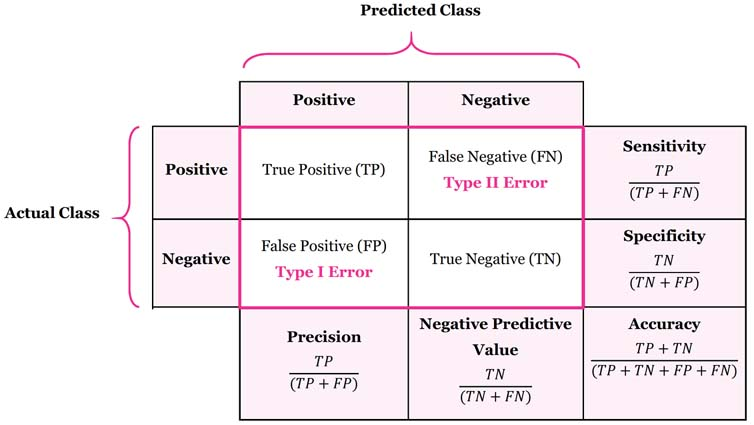
\includegraphics[width=0.8\textwidth]{figs/confusionMatrix.jpg}
    \label{fig:confusionMatrix}
    \caption{Macierz pomyłek oraz możliwe metryki oceny jakości klasyfikatora}
\end{figure}

Wartość precision określa jak pewny jest klasyfikator przy wykrywaniu klasy pozytywnej, natomiast
recall mówi o tym jak dobrze klasyfikator \enquote{wyławia} przykłady pozytywne. Zauważmy jednak, iż
nie możemy stosować żadnej z tych metryk w odosobnieniu. Istotnie klasyfikator, który zwraca zawsze
klasę pozytywną ma maksymalny recall, a klasyfikator, który zwraca zawsze klasę negatywną ma
nieokreślony precision (i jest oczywiście beznadziejnym klasyfikatorem). Musimy więc zawsze
ewaluować model na obu tych metrykach i jedynie dobry wynik obu z nich mówi o jakości klasyfikatora.
Oczywiście czasami chcielibyśmy określić jakość modelu za pomocą jednej liczby, a niekoniecznie
sprawdzać zawsze macierz pomyłek (choć jest to bardzo użyteczne) lub podawać wartości dwóch metryk.
Metryką, która łączy precision i recall jest \emph{\(F_\beta\)--score} zdefiniowany jako
\begin{equation}
    F_\beta := (1 + \beta^2) \frac{\mathrm{Precision} \cdot \mathrm{Recall}}{\beta^2 \cdot \mathrm{Precision} + \mathrm{Recall}}\,, 
\end{equation}
gdzie \(\beta\) określa ile razy bardziej ważny jest recall od precision. Typowo używa się
\(F_1\)--score
\begin{equation}
    F_1 = 2\frac{\mathrm{Precision} \cdot \mathrm{Recall}}{\mathrm{Precision} + \mathrm{Recall}}\,. 
\end{equation}

Wiele klasyfikatorów oprócz twardych predykcji zwraca również rozkład prawdopodobieństwa nad
klasami. W przypadku klasyfikacji binarnej jest to oczywiście rozkład zero-jedynkowy z parametrem
\(p\) określającym prawdopodobieństwo klasy pozytywnej dla danego wektora cech. Standardowo
oczywiście twardą predykcją jest ta z klas, która ma większe prawdopodobieństwo, czyli (co
równoważne) predykcją jest klasa pozytywna jeśli \(p > 0.5\). W niektórych problemach chcemy jednak
zmienić ten próg i dokonać tzw. \textit{threshold tuning}. Wykresem, który pozwala na dokonanie
tuningu progu jest \emph{krzywa ROC} (z ang. \textit{Receiver Operatic Characteristic curve}), która
jest krzywą parametryczną wyznaczoną przez punkty \((\mathrm{FPR}(\mathrm{threshold}),
\mathrm{TPR}(\mathrm{threshold}))\) dla progów z zakresu \([0;1]\), gdzie
\begin{equation}
    \mathrm{TPR} := \frac{\mathrm{TP}}{\mathrm{TP + FN}}\,,\quad \mathrm{FPR} := \frac{\mathrm{FP}}{\mathrm{FP + TN}}\,.
\end{equation}
Metryką niezależną od wybranego progu jest tzw. \emph{AUROC} (z ang. \textit{Area under ROC curve})
zdefiniowany jako pole powierzchni pod krzywą ROC dla danego klasyfikatora. Zauważmy, że
klasyfikator losowy, który zwraca zawsze klasę pozytywną z prawdopodobieństwem równym wartości progu
ma wartość AUROC równą 0.5, natomiast idealny klasyfikator, który niezależnie od wartości progu
klasyfikuje wszystkie przykłady poprawnie ma AUROC równy 1.

Inną analogiczną metryką jest \emph{AUPRC}, gdzie zamiast krzywej ROC stosujemy krzywą \emph{PRC} (z
ang. \textit{Precision--Recall Curve}), w której zamiast TPR i FPR używamy odpowiednio Precision i
Recall. Metryka AUPRC jest często wykorzystywana w przypadku klasyfikacji ekstremalnie
niezbalansowanej, w której mamy bardzo mało (< 1\%) klasy pozytywnej.


\subsubsection{Klasyfikacja wieloklasowa}

W przypadku klasyfikacji wieloklasowej używamy zasadniczo takich samych metryk jak w klasyfikacji
binarnej, ale wprowadzamy mikro i makro uśrednianie (z ang. \textit{micro/macro-averaging}). Przez
\(\mathrm{TP}_k\) będziemy rozumieć liczbę prawidłowo zaklasyfikowanych przykładów z klasy \(k\),
\(\mathrm{FP}_k\) to liczba przykładów z innych klas, które zaklasyfikowaliśmy nieprawidłowo jako
\(k\)--tą klasę, \(\mathrm{FN}_k\) to liczba przykładów z klasy \(k\), które zaklasyfikowaliśmy jako
inną klasę. Wówczas odpowiednie metryki mają postać
\begin{equation}
    \begin{split}
        &\mathrm{MicroPrecision} := \frac{\sum_{k} \mathrm{TP}_k}{\sum_{k} \mathrm{TP}_k + \sum_{k} \mathrm{FP}_k}\,,\\
        &\mathrm{MacroPrecision} := \frac{1}{K} \sum_{k=1}^K \frac{\mathrm{TP}_k}{\mathrm{TP}_k + \mathrm{FP}_k}
    \end{split}
\end{equation}
oraz
\begin{equation}
    \begin{split}
        &\mathrm{MicroRecall} := \frac{\sum_{k} \mathrm{TP}_k}{\sum_{k} \mathrm{TP}_k + \sum_{k} \mathrm{FN}_k}\,,\\
        &\mathrm{MacroRecall} := \frac{1}{K} \sum_{k=1}^K \frac{\mathrm{TP}_k}{\mathrm{TP}_k + \mathrm{FN}_k}\,.
    \end{split}
\end{equation}
W przypadku klasyfikacji wieloklasowej macierz pomyłek jest macierzą wymiaru \(K \times K\), gdzie
\(K\) jest liczbą klas.


\subsection{Klasyfikator najbliższych sąsiadów}

Do tej pory zajmowaliśmy się problemami regresji ciągłej zmiennej skalarnej. Przechodzimy teraz do
metod uczenia maszynowego wykorzystywanych dla problemów klasyfikacji. Jako pierwszy rozważmy jeden
z najprostszych (ale bardzo mocnych) modeli -- klasyfikator \(k\) najbliższych sąsiadów (z ang.
\textit{k Nearest Neighbors, kNN}). Załóżmy, iż mamy zbiór obserwacji i.i.d. postaci \(\mathcal{X} =
\{y_i(\bm{x}_i)\}_{i=1}^n\) przy czym \(y\) może być zarówno skalarną zmienną ciągłą jak i elementem
skończonego zbioru klas. Zakładamy, że wektory cech \(\bm{x} \in \mathbb{R}^d\), a \(\mathsf{d}:
\mathbb{R}^d \times \mathbb{R}^d \mapsto I \subseteq \mathbb{R}\) jest metryką, półmetryką lub pewną
miarą podobieństwa między punktami \(\mathbb{R}^d\). Reguła decyzyjna klasyfikatora \(k\)
najbliższych sąsiadów polega na znalezieniu dla nowego wektora cech \(\bm{t}\), \(k\) najbliższych
względem funkcji \(\mathsf{d}\) punktów ze zbioru \(\{\bm{x}_1,\ldots,\bm{x}_n\}\) i zwróceniu
najczęstszej klasy dla tych sąsiadów. Metodę najbliższych sąsiadów można również wykorzystać do
regresji, gdzie zwracamy wartość średnią arytmetyczną wartości \(y\) dla znalezionych \(k\)
najbliższych sąsiadów (powoduje to, że model taki potrafi tylko interpolować wartości, więc nie jest
dobrym modelem dla regresji). W przypadku klasyfikacji możemy natomiast zwracać również rozkład
prawdopodobieństwa klas dla nowego wektora cech \(\bm{t}\) przez podanie stosunków występowania
danej klasy wśród \(k\) najbliższych sąsiadów do \(k\).

Klasyfikator kNN jest bardzo elastycznym modelem z nieliniową granicą decyzyjną. Jakość klasyfikacji
silnie zależy od lokalnej gęstości punktów w przestrzeni \(\mathbb{R}^d\) oraz wybranej wartości
\(k\), będącej hiperparametrem tego modelu. Ogólnie niskie \(k\) powoduje, że kNN ma duży variance i
dość \enquote{poszarpaną} granicę decyzyjną, natomiast wysokie \(k\) powoduje, że kNN ma duży bias i
\enquote{gładką} granicę decyzyjną. Typowo wykorzystywane funkcje \(\mathsf{d}\) to
\begin{itemize}
    \item metryka euklidesowa \(\mathsf{d}(\bm{x},\bm{y}) = \sqrt{(\bm{x} - \bm{y})^T(\bm{x} -
    \bm{y})}\);

    \item pół-metryka euklidesowa \(\mathsf{d}(\bm{x},\bm{y}) = (\bm{x} - \bm{y})^T(\bm{x} -
    \bm{y})\);

    \item metryka Manhattan \(\mathsf{d}(\bm{x}, \bm{y}) = \sum_{i=1}^d |\bm{x}^i - \bm{y}^i|\);
    
    \item podobieństwo cosinusowe \(\mathsf{d}(\bm{x}, \bm{y}) =
    \frac{\bm{x}^T\bm{y}}{\norm{\bm{x}}_2 \norm{\bm{y}}_2}\)
\end{itemize}

Jedną z modyfikacji klasyfikatora kNN, który może polepszyć wyniki w przypadku, gdy w naszej
przestrzeni istnieją obszary, w których mamy małą gęstość punktów ze zbioru \(\mathcal{X}\) jest
\emph{ważenie sąsiadów}, które polega na tym, iż prawdopodobieństwa danej klasy wśród \(k\) sąsiadów
obliczamy teraz jako średnią ważoną, gdzie wagą jest odwrotność odległości danego sąsiada od nowego
wektora cech \(w(\bm{t}, \bm{x}) = 1 / \mathsf{d}(\bm{t}, \bm{x})\).

W przypadku naiwnego kNN podczas treningu zapamiętujemy jedynie zbiór \(\mathcal{X}\) natomiast
naiwna implementacja predykcji ma złożoność czasową \(O(knd)\), przy założeniu, że złożoność
obliczenia funkcji \(\mathsf{d}\) dla pary punktów ma złożoność \(O(d)\). Jest to nieakceptowalna
złożoność, gdyż zwykle chcemy używać klasyfikatora kNN do setek milionów punktów. Dwa podejścia,
które stosuje się zwykle do rozwiązania tego problemu to: 
\begin{itemize}

    \item zbudowanie odpowiedniej struktury danych w fazie treningu, aby w czasie predykcji można
    było szybciej znajdywać najbliższych sąsiadów (np. k-d tree, ball tree);

    \item wykorzystanie algorytmów aproksymacyjnych (z ang. \textit{Approximate Nearest Neighbors,
    ANN}) do znajdowania sąsiadów, którzy niekoniecznie naprawdę są najbliżsi, ale aproksymacja jest
    wystarczająco dobra do praktycznych zastosowań.

\end{itemize}

Obecnie to drugie podejście jest dominujące i wykorzystywane na przykład w przypadku dużych modeli
językowych do wyszukiwania kontekstów dla danych zapytań (z ang. \textit{Retrieval Augmented
Generation}).


\subsection{Naiwny klasyfikator bayesowski}

Rozważamy dalej problem klasyfikacji, w którym mamy zbiór przykładów i.i.d. postaci \(\mathcal{X} =
\{y_i(\bm{x}_i)\}_{i=1}^n\), gdzie \(y \in \{c_1, \ldots, c_K\} \) oraz \(\bm{x} \in \mathbb{R}^d\).
W ogólności mamy rozkład warunkowy danej klasy pod warunkiem wektora cech, który jest dany przez
gęstość prawdopodobieństwa \(p(c_k \mid \bm{x})\). Korzystając z twierdzenia Bayesa możemy zapisać
\begin{equation}
    p(c_k \mid \bm{x}) = \frac{p(\bm{x} \mid c_k) p(c_k)}{p(\bm{x})}\,.
\end{equation}
Jeśli umiemy obliczyć licznik wyrażenia po prawej stronie, to korzystając z \emph{reguły decyzyjnej
MAP} klasę dla nowego wektora cech wybieramy jako
\begin{equation}
    \arg\max_{c_k \in \{c_1, \ldots, c_K\}} p(\bm{x} \mid c_k) p(c_k)\,.
\end{equation}
Powstaje pytanie jak obliczyć to wyrażenie przy tak luźnych założeniach. Wprowadzamy naiwne
założenie warunkowej niezależności cech względem danej klasy tj.
\begin{equation}
    p(\bm{x} \mid c_k) = p(\bm{x}^1, \ldots, \bm{x}^d \mid c_k) = \prod_{j=1}^d p(\bm{x}^j \mid c_k)\,.
\end{equation}
Teraz jednowymiarowe rozkłady warunkowe \(p(\bm{x}^j \mid c_k)\) możemy estymować z danych
\(\mathcal{X}\) np. korzystając z jądrowego estymatora gęstości lub zakładając konkretny model
parametryczny (np. jednowymiarowy rozkład normalny, rozkład dwumianowy) i estymując jego parametry
dla każdej z klas osobno. Naiwne założenie warunkowej niezależności pozwala złagodzić problemy
wynikające z przekleństwa wymiarowości (z ang. \textit{curse of dimensionality}), takie jak potrzeba
zbiorów danych skalujących się wykładniczo wraz z liczbą cech \(d\). Człon \(p(c_k)\) można
natomiast prosto oszacować jako stosunek przykładów danej klasy w zbiorze \(\mathcal{X}\).


\subsection{Estymator jądrowy gęstości}

Załóżmy, że mamy zbiór obserwacji i.i.d. \(\{\bm{x}_1, \ldots, \bm{x}_n\}\) taki, że \(\bm{x} \sim
\mathcal{D}\) dla pewnego \(d\)--wymiarowego ciągłego rozkładu prawdopodobieństwa \(\mathcal{D}\) z
nieznaną gęstością prawdopodobieństwa \(p(\bm{x})\). Chcemy znaleźć estymator \(\hat{p}(\bm{x})\)
tej funkcji. Estymatorem jądrowym gęstości funkcji \(p\) (z ang. \textit{kernel density estimator})
nazywamy funkcję
\begin{equation}\boxed{
    \hat{p}(\bm{x}) := \frac{1}{mh^d}\sum_{i=1}^n K\left(\frac{\bm{x} - \bm{x}_i}{h}\right)\,,
}\end{equation}
gdzie \(h \in \mathbb{R}\) jest pewnym hiperparametrem zwanym \textit{bandwidth}, a \(K:
\mathbb{R}^d \mapsto [0; \infty)\) to tzw. funkcja jądrowa będąca parzystą funkcją posiadającą w 0
maksimum globalne oraz spełniającą warunek unormowania
\begin{equation}
    \int\limits_{\mathbb{R}^d} K(\bm{x}) \dd[d]{\bm{x}}= 1\,.
\end{equation}
Ze statystycznego punktu widzenia, postać jądra nie ma istotnego znaczenia i wybór funkcji  \(K\)
może być arbitralny, uwzględniający przede wszystkim pożądane własności otrzymanego estymatora, na
przykład klasę jego regularności (ciągłość, różniczkowalność itp.). W przypadku jednowymiarowym jako
funkcję \(K\) przyjmuje się klasyczne postacie gęstości rozkładów probabilistycznych, na przykład
gęstość rozkładu normalnego. W przypadku wielowymiarowym stosuje się tzw. jądro radialne tj. dla
jądra jednowymiarowego \(K\) wielowymiarowe jądro radialne definiujemy jako
\begin{equation}
    K(\bm{x}) = K(\norm{\bm{x}})
\end{equation}
dla pewnej normy (typowo normy euklidesowej) \(\norm{\cdot}\).

KDE w praktycznych zastosowaniach często przyspiesza się za pomocą struktur danych analogicznych jak
w przypadku kNN, tj. zamiast sumować przyczynki od wszystkich punktów \(\bm{x}_i\) dla danego
\(\bm{x}\), znajdujemy \(k\) najbliższych sąsiadów \(\bm{x}\) ze zbioru \(\{\bm{x}_i\}_{i=1}^n\)
stosując np. ANN i obliczamy przyczynki do \(\hat{p}(\bm{x})\) tylko od nich.

Jedynym większym problemem w przypadku KDE jest wybór odpowiedniej wartości parametru \(h\). Jeśli
używamy jądra gaussowskiego to \emph{reguła Silvermana}, która podaje prosty przepis na szerokość
kernela, przy założeniu, iż rozkład jest unimodalny
\begin{equation}
    h_\mathrm{Silverman} = \left(\frac{4}{d + 2}\right)n^{\frac{-1}{d + 4}}\sigma\,,
\end{equation}
gdzie \(\sigma\) to odchylenie standardowe, \(n\) to liczba próbek, a \(d\) -- liczba wymiarów.


\subsection{Wieloklasowa regresja logistyczna}

Powróćmy do zagadnienia klasyfikacji, w którym mamy zbiór obserwacji i.i.d. \(\mathcal{X} =
\{y_i(\bm{x}_i)\}_{i=1}^n\), gdzie \(y \in \{c_1,\ldots,c_K\}\) i \(\bm{x} \in \mathbb{R}^d\).
Pokażemy teraz podejście oparte na estymacji MLE podobnie jak w przypadku regresji. Założymy, że
obserwacje \(y(\bm{x})\) pochodzą z rozkładu kategorialnego (wielopunktowego) zależnego od
parametrów \(\bm{W}\) jako
\begin{equation}
    y(\bm{x}) \mid \bm{W} \sim \mathrm{Cat}\left(\bm{\pi}^1(\bm{\phi}(\bm{x}; \bm{W})), \ldots, \bm{\pi}^K(\bm{\phi}(\bm{x}; \bm{W}))\right)\,,
\end{equation}
gdzie funkcja \(\bm{\pi}: \mathbb{R}^K \mapsto [0;1]^K\) musi spełniać warunek unormowania
\begin{equation*}
    \forall \bm{z}\in\mathbb{R}^K: \sum_{j=1}^K \bm{\pi}^j(\bm{z}) = 1\,,
\end{equation*}
aby jej składowe były odpowiadały prawdopodobieństwom danej klasy, Funkcja \(\bm{\phi}: \mathbb{R}^d
\mapsto \mathbb{R}^K\) jest natomiast dowolną funkcją przekształcającą wektor cech na rzeczywisty
wektor wymiaru \(K\). W szczególności przyjmiemy następującą postać funkcji \(\bm{\pi}\) zwaną
\emph{funkcją softmax}
\begin{equation}\boxed{
    \bm{\pi}^j(\bm{z}) = \frac{\exp\left(\bm{z}^j\right)}{\sum_{k=1}^K \exp\left(\bm{z}^k\right)}\,.
}\end{equation}
W przypadku wieloklasowej regresji logistycznej (zwanej również \emph{regresją softmax}) jako
funkcję \(\bm{\phi}\) przyjmiemy proste przekształcenie liniowe
\begin{equation}
    \bm{\phi}(\bm{x}; \bm{W}) = \bm{W}\bm{x}\,,
\end{equation} 
gdzie \(\bm{W}\) jest macierzą estymowanych parametrów wymiaru \(K \times d\). Wyprowadzimy teraz
wzór na funkcję kosztu przy takim modelu statystycznym. Zauważmy wpierw, iż wiarygodność
pojedynczego przykładu ze zbioru \(\mathcal{X}\) możemy zapisać jako
\begin{equation}
    p(y_i(\bm{x}_i) \mid \bm{W}) = \prod_{j=1}^K \bm{\pi}^j\left(\bm{\phi}(\bm{x}_i; \bm{W})\right)^{[y_i = c_j]}\,,
\end{equation}
gdzie \([\ldots]\) oznacza nawias Iversona. W takim razie wiarygodność całego zbioru \(\mathcal{X}\)
ma postać
\begin{equation}
    \mathcal{L}(\mathcal{X}; \bm{W}) = \prod_{i=1}^n \prod_{j=1}^K \bm{\pi}^j\left(\bm{\phi}(\bm{x}_i; \bm{W})\right)^{[y_i = c_j]}\,,
\end{equation}
skąd funkcja kosztu ma postać
\begin{equation}
    L(\mathcal{X}; \bm{W}) = - \sum_{i=1}^n \sum_{j=1}^K [y_i = c_j] \log \left[ \bm{\pi}^j\left(\bm{\phi}(\bm{x}_i; \bm{W})\right)\right]\,.
\end{equation}
Wprowadzając macierze 
\begin{equation*}
    \begin{split}
        &\bm{X}^{ij} = \bm{x}_j^i\,,\quad \bm{X} = \mqty[\bm{x}_1 & \ldots & \bm{x_n}]\\
        &\bm{T}^{ij} = [y_j = c_i]\\
        &\bm{\Phi}^{ij}(\bm{X}; \bm{W}) = \bm{\phi}^i(\bm{x}_j;\bm{W}) = \sum_{k=1}^d \bm{W}^{ik}\bm{X}^{kj}\,,\quad \bm{\Phi}(\bm{X};\bm{W}) = \bm{W}\bm{X}\\
        &\bm{\Pi}^{ij}(\bm{\Phi}) = \bm{\pi}^i\left(\bm{\phi}(\bm{x}_j;\bm{W})\right) = \frac{\exp\bm{\Phi}^{ij}}{\sum_{k=1}^K \exp \bm{\Phi}^{kj}}
    \end{split}
\end{equation*}
gdzie każda kolumna macierzy \(\bm{X}\) jest wektorem cech danego przykładu; każda kolumna
\(\bm{T}\) jest tzw. \emph{wektorem one--hot} dla danego przykładu tj. wektorem binarnym, w którym
dokładnie na jednej pozycji jest wartość 1 i pozycja ta odpowiada prawidłowej klasie dla danego
przykładu; każda kolumna macierzy \(\bm{\Phi}\) jest wektorem \emph{mlogitów} tj. liczb
rzeczywistych, które po zastosowaniu funkcji softmax dają wartości prawdopodobieństwa każdej klasy;
możemy zapisać
\begin{equation}\boxed{
    L(\mathcal{X}; \bm{W}) = -\sum_{j=1}^n\sum_{i=1}^K \bm{T}^{ij} \log \left[ \bm{\Pi}^{ij}(\bm{\Phi}(\bm{X}; \bm{W})) \right]\,.
}\end{equation}

Niestety dla tak zdefiniowanej funkcji kosztu nie można znaleźć wzoru na minimum w postaci
analitycznej (jak w przypadku regresji liniowej), dlatego do znalezienia estymaty MLE wykorzystujemy
algorytmy optymalizacji numerycznej, w tym przypadku zwykle algorytmy gradientowe. Wyprowadzimy więc
jeszcze wzór na pochodną funkcji kosztu po parametrach \(\bm{W}\). Obliczmy najpierw pochodną \(L\)
po \(\bm{\Phi}^{ij}\) (dla przejrzystości zapisu nie piszemy granic sumowania -- wynikają one
naturalnie z wymiarów macierzy)
\begin{equation}
    \pdv{L}{\bm{\Phi}^{pq}} = -\sum_{i,j,r,s} \frac{\bm{T}^{ij}}{\bm{\Pi}^{rs}}\delta_{ir}\delta_{js}\pdv{\bm{\Pi}^{rs}}{\bm{\Phi}^{pq}} = - \sum_{i,j} \frac{\bm{T}^{ij}}{\bm{\Pi}^{ij}}\pdv{\bm{\Pi}^{ij}}{\bm{\Phi}^{pq}}\,.
\end{equation}
Jednocześnie
\begin{equation}
    \pdv{\bm{\Pi}^{ij}}{\bm{\Phi}^{pq}} = \frac{\delta_{pi}\delta_{qj}\exp\bm{\Phi}^{ij}\left[\sum_k \exp\bm{\Phi}^{kj}\right] - \delta_{qj} \exp\bm{\Phi}^{ij} \exp\bm{\Phi}^{pj}}{\left[\sum_k \exp\bm{\Phi}^{kj}\right]^2}\,,
\end{equation}
skąd
\begin{equation}
    \frac{1}{\bm{\Pi}^{ij}}\pdv{\bm{\Pi}^{ij}}{\bm{\Phi}^{pq}} = \delta_{pi}\delta_{qj} - \delta_{qj}\bm{\Pi}^{pj}\,.
\end{equation}
Z powyższego zatem
\begin{equation}
    \pdv{L}{\bm{\Phi}^{pq}} = -\sum_{i,j} \bm{T}^{ij}\delta_{pi}\delta_{qj} + \sum_{i,j}\bm{T}^{ij}\delta_{qj}\bm{\Pi}^{pj} = \bm{\Pi}^{pq} - \bm{T}^{pq}\,,
\end{equation}
gdzie skorzystaliśmy z faktu, iż z konstrukcji dla dowolnej kolumny \(q\) macierzy \(\bm{T}\)
zachodzi \(\sum_{i}\bm{T}^{iq} = 1\). Możemy zapisać powyższy wzór w eleganckiej postaci macierzowej
\begin{equation}\boxed{
    \pdv{L}{\bm{\Phi}} = \bm{\Pi} - \bm{T}\,.
}\end{equation}
Pochodną funkcji kosztu po parametrach \(\bm{W}\) możemy zatem obliczyć jako
\begin{equation}
    \pdv{L}{\bm{W}^{rs}} = \sum_{p,q}\pdv{L}{\bm{\Phi}^{pq}}\pdv{\bm{\Phi}^{pq}}{\bm{W}^{rs}}\,,
\end{equation}
gdzie
\begin{equation}
    \pdv{\bm{\Phi}^{pq}}{\bm{W}^{rs}} = \sum_t \delta_{rp} \delta_{st} \bm{X}^{tq} = \delta_{rp}\bm{X}^{sq}\,,
\end{equation}
skąd
\begin{equation}
    \pdv{L}{\bm{W}^{rs}} = \sum_{q} (\bm{\Pi}^{rq} - \bm{T}^{rq}) \bm{X}^{sq}\,,
\end{equation}
co również możemy zapisać w zwartej postaci macierzowej
\begin{equation}\boxed{
    \pdv{L}{\bm{W}} = (\bm{\Pi} - \bm{T}) \bm{X}^T\,.
}\end{equation}


\subsection{Metody selekcji cech}

Zwykle dane w zbiorach wykorzystywanych w uczeniu maszynowym mają dużą wymiarowość (wiele cech). Nas
jednak najbardziej interesuje tzw. \textit{intrinsic dimensionality}, czyli podprzestrzeń, która
jest realnie ważna dla problemu klasyfikacji lub regresji. Celem selekcji cech jest właśnie wybór
tych cech, które są istotne. Typowo obliczamy ważność cech (z ang. \textit{feature importance}) i
usuwamy te najmniej wartościowe. Takie podejście może pomóc nam usunąć szum z danych i poprawić
wyniki modeli (jest to szczególne ważne dla modeli, które używają cech wprost np. kNN, Naive Bayes).
Najczęstszymi podejściami do selekcji cech są tzw. metody \textit{filter} i \textit{embedded}.
\begin{itemize}
    
    \item \emph{Metody \textit{filter}}. Waga cechy jest obliczana na podstawie pewnej ogólnej miary
    jakości cech; są typowo oparte na pewnych statystykach i sprawdzają pojedynczą zmienną naraz
    (tzw. metody \textit{univariate}).
    
    \begin{itemize}

        \item \emph{\textit{Variance threshold}}. Przeskalowujemy cechy korzystajac z MinMax, aby
        wszystkie miały ten sam zakres wartości. Obliczamy wariancję każdej cechy. Odrzucamy cechy o
        bardzo małej wariancji, oznacza to bowiem, iż są praktycznie stałe. Próg typowo jest
        ustalany na bardzo niski typu 0.01.

        \item \emph{Korelacja cech}. Obliczamy macierz korelacji i cech, po czym z każdej pary
        eliminujemy najmocniej skorelowane cechy, poprzez usunięcie tej o niższej wariancji lub tej,
        która ma średnio większe korelacje z innymi cechami.

        \item \emph{Korelacja ze zmienną zależną}. Obliczamy korelacje między cechami, a zmienną
        zależną i usuwamy te o wartości bezwzględnej bliskiej 0. 

        \item \emph{\textit{Mutual Information}}. Obliczamy informację wzajemną (z ang.
        \textit{Mutual Information, MI}) zdefiniowaną dla zmiennych losowych rzeczywistych \(X, Y\),
        jako
        \begin{equation}
            I(X; Y) = \iint p(x, y) \log\left[\frac{p(x,y)}{p(x)p(y)}\right] \dd{x}\dd{y}\,.
        \end{equation}
        Gdy zmienne są niezależne, to MI wynosi 0. Aby obliczyć powyższy wzór używamy KDE i
        najbliższych sąsiadów, aby przybliżyć rozkłady prawdopodobieństwa.

    \end{itemize}

    \item \emph{Metody \textit{embedded}}. W metodach embedded trenujemy jakiś parametryczny model
    uczenia maszynowego na naszych danych i wagi tego modelu interpretujemy jako wagi cech w
    zbiorze. Metody te wymagają dobrych modeli, zauważmy bowiem, że wagi modelu mówią tak naprawdę
    jak ważna jest dana cecha dla predykcji tego modelu, a nie ogólnie dla zagadnienia. Jako modele
    można wybrać proste modele liniowe, w których mamy prostą interpretację wag.

\end{itemize}


\subsection{Próbkowanie Monte Carlo łańcuchami Markowa}

Okazuje się, iż do generowania próbek ze skomplikowanego rozkładu \(p(\bm{x})\) wystarcza znajomość
tego rozkładu z dokładnością do stałej normalizującej, a zatem wystarczy znać rozkład łączny
\(\tilde{p}(\bm{x}) = Z_p p(\bm{x})\). Generowanie próbek z kolei wystarcza natomiast, na mocy
silnego prawa wielkich liczb, do szacowania wartości średnich dowolnych funkcji estymowanego
parametru \(\theta\). Przypomnijmy, iż na mocy silnego prawa wielkich liczb ciąg średnich
częściowych \((\overline{X}_n)\) ciągu zmiennych losowych \((X_n)\) i.i.d. z rozkładu \(X \sim
\mathcal{D}\) jest zbieżny z prawdopodobieństwem 1 do wartości oczekiwanej \(\mathbb{E}[X]\) tj.
\begin{equation}
    \Pr\left(\lim_{n \to \infty} \overline{X}_n = \mathbb{E}[X]\right) = 1\,.
\end{equation}
Wartość oczekiwaną \(\mathbb{E}[X]\) możemy zatem przybliżyć średnią \(\overline{X}_n\) z dużej
ilości próbek.

Pozostaje pytanie w jaki sposób generować próbki ze skomplikowanych rozkładów prawdopodobieństwa,
których gęstości znamy jedynie z dokładnością do stałej normalizującej. Poniżej przedstawimy dwa
algorytmy próbkowania: algorytm IS oraz Metropolisa--Hastingsa będący szczególną realizacją całej
rodziny algorytmów próbkowania zwanych Markov Chain Monte Carlo (MCMC).

\subsubsection{Algorytm Importance Sampling}

Załóżmy, iż chcemy obliczyć wartość oczekiwaną pewnej funkcji zmiennej losowej \(\bm{x}\) względem
skomplikowanego rozkładu prawdopodobieństwa \(p(\bm{x})\), który znamy jedynie z dokładnością do
stałej normalizującej
\begin{equation}
    p(\bm{x}) = \frac{1}{Z_p}\tilde{p}(\bm{x})
\end{equation}
tj. szukamy
\begin{equation}
    \mathbb{E}_p[f(\bm{x})] = \int f(\bm{x}) p(\bm{x})\dd[n]\bm{x}\,.
\end{equation}
Jeśli umiemy generować próbki \(\bm{x}\) z innego (prostszego) rozkładu \(q(\bm{x})\), który
nazywamy rozkładem proponującym kandydatów (z ang. \textit{proposal distribution}) to możemy zapisać
\begin{equation}
    \begin{split}
        \mathbb{E}_p[f(\bm{x})] &= \int\limits_{\mathbb{R}^n}f(\bm{x})p(\bm{x})\dd[n]\bm{x} = \int\limits_{\mathbb{R}^n}f(\bm{x})\frac{p(\bm{x})}{q(\bm{x})}q(\bm{x})\dd[n]\bm{x}\\
         &=\mathbb{E}_q\left[f(\bm{x}) \frac{p(\bm{x})}{q(\bm{x})}\right] = \frac{Z_q}{Z_p}\mathbb{E}_q\left[f(\bm{x}) \frac{\tilde{p}(\bm{x})}{\tilde{q}(\bm{x})}\right]\,.
    \end{split}
\end{equation}
Zakładamy tutaj, iż nośnik rozkładu \(p\) zawiera się w nośniku \(q\) tj. \(\text{supp}\,p \subseteq
\text{supp}\,q\). Stosunek stałych \(Z_p / Z_q\) również możemy oszacować z próbek z \(q\), gdyż
mamy
\begin{equation}
    Z_p = \int\limits_{\mathbb{R}^n}\tilde{p}(\bm{x})\dd[n]{\bm{x}} = Z_q\int\limits_{\mathbb{R}^n}\frac{\tilde{p}(\bm{x})}{\tilde{q}(\bm{x})} q(\bm{x})\dd[n]{\bm{x}} = Z_q \mathbb{E}_q\left[\frac{\tilde{p}(\bm{x})}{\tilde{q}(\bm{x})}\right]\,,
\end{equation}
skąd ostatecznie
\begin{equation}
    \mathbb{E}_p[f(\bm{x})] = \frac{\mathbb{E}_q\left[f(\bm{x}) \frac{\tilde{p}(\bm{x})}{\tilde{q}(\bm{x})}\right]}{\mathbb{E}_q\left[\frac{\tilde{p}(\bm{x})}{\tilde{q}(\bm{x})}\right]}\,.
\end{equation}
Jeśli z rozkładu \(q\) wygenerowaliśmy próbki \(X = \left\{\bm{x}_1,\ldots,\bm{x}_m\right\}\) to na
mocy silnego prawa wielkich liczb mamy
\begin{equation}\boxed{
    \mathbb{E}_p[f(\bm{x})] \approx \frac{\sum_{i=1}^m f(\bm{x}_i) \frac{\tilde{p}(\bm{x}_i)}{\tilde{q}(\bm{x}_i)}}{\sum_{j=1}^m \frac{\tilde{p}(\bm{x}_j)}{\tilde{q}(\bm{x}_j)}} = \sum_{i=1}^m \lambda_i f(\bm{x}_i)\,,
}\end{equation}
gdzie
\begin{equation}\boxed{
    \lambda_i = \frac{\tilde{p}(\bm{x}_i) / \tilde{q}(\bm{x}_i)}{\sum_{j=1}^m \tilde{p}(\bm{x}_j) / \tilde{q}(\bm{x}_j) }\,.
}\end{equation}

Algorytm Importance Sampling jest prostym algorytmem Monte Carlo, który ma jeden zasadniczy problem.
W jaki sposób mamy wybrać rozkład proponujący kandydatów \(q\)? Pewną odpowiedź na to pytanie
sugeruje analiza wariancji statystyki 
\begin{equation}
    \overline{f}_m(\bm{x}_1,\ldots,\bm{x}_m) = \frac{1}{m}\sum_{i=1}^m \frac{f(\bm{x}_i)p(\bm{x}_i)}{q(\bm{x}_i)}
\end{equation}
dla \(\bm{x}_i \sim q\) mamy
\begin{equation}
    \begin{split}
        \mathbb{V}[\overline{f}_m] &= \frac{1}{m}\mathbb{V}_q\left[f(\bm{x})\frac{p(\bm{x})}{q(\bm{x})}\right] = \frac{1}{m}\int\limits_{\mathbb{R}^n}\frac{(f(\bm{x})p(\bm{x}) - \mu_fq(\bm{x}))^2}{q(\bm{x})}\dd[n]{\bm{x}}\,.
    \end{split}
\end{equation}
Chcemy oczywiście, aby wariancja była jak najmniejsza, gdyż wówczas mała liczba próbek da dobre
przybliżenie wartości oczekiwanej. Rozkład proponujący kandydatów powinien być zatem proporcjonalny
do \(f(\bm{x})p(\bm{x})\), co może być trudne do praktycznego zrealizowania.


\subsubsection{Algorytm Metropolisa--Hastingsa}

Cała klasa algorytmów próbkowania MCMC opiera się na idei wyrażenia generowania próbek jako ewolucji
pewnego łańcucha Markowa.

\begin{definition}[Łańcucha Markowa]
Łańcuchem Markowa nazwiemy ciąg zmiennych losowych \((\bm{X}_t)\) o wartościach w \(\mathbb{R}^n\)
taki, że spełnione jest \emph{kryterium Markowa}
\begin{equation*}
    \begin{split}
        \forall A \subset \mathbb{R}^n :\, &\Pr(\bm{X}_t \in A \mid \bm{X}_{t-1} = \bm{x}_{t-1}, \ldots, \bm{X}_0 = \bm{x}_0) \\
        &= \Pr(\bm{X}_t \in A \mid \bm{X}_{t-1} = \bm{x}_{t-1})\,.
    \end{split}
\end{equation*}
Elementy ciągu nazywamy stanami łańcucha.
\end{definition}

Dany łańcuch jest zadany jednoznacznie przez podanie gęstości prawdopodobieństwa przejścia łańcucha
ze stanu \(\bm{x} \to \bm{y}\), którą będziemy oznaczać przez \(\pi(\bm{y} \mid \bm{x})\)
(zakładamy, iż prawdopodobieństwo przejścia jest niezależne od chwili \(t\) -- łańcuch taki nazywamy
jednorodnym). Funkcja \(\pi\) spełnia oczywiście warunek unormowania
\begin{equation}
    \int\limits_{\mathbb{R}^n} \pi(\bm{y} \mid \bm{x}) \dd[n]{\bm{y}}\,,
\end{equation} 
istotnie prawdopodobieństwo przejścia gdziekolwiek ze stanu \(\bm{x}\) jest równe 1. Będziemy
zakładać dodatkowo, iż \(\forall \bm{x},\bm{y}\in\mathbb{R}^n: \pi(\bm{y} \mid \bm{x}) > 0\).
Rozkład \(p(\bm{x})\) łańcucha Markowa (tj. rozkład prawdopodobieństwa z którego losujemy stan
łańcucha w danej chwili \(t\)) z daną funkcją przejścia \(\pi\) nazwiemy rozkładem stacjonarnym tego
łańcucha jeśli
\begin{equation}
    p(\bm{y}) = \int\limits_{\mathbb{R}^n} \pi(\bm{y} \mid \bm{x})p(\bm{x}) \dd[n]{\bm{x}}\,.
\end{equation}
Rozkład stacjonarny danego łańcucha oznaczymy przez \(p^*(\bm{x})\). Zauważmy, iż jeśli stan
początkowy łańcucha \(\bm{X}_0\) pochodzi z rozkładu stacjonarnego \(p^*\) to każdy kolejny stan
\(\bm{X}_t\) również pochodzi z rozkładu stacjonarnego. Jeśli z kolei stan początkowy pochodzi z
jakiegoś innego rozkładu \(p_0\) to rozkład łańcucha w chwili \(t\) jest dany przez relację
rekurencyjną
\begin{equation}
    p_t(\bm{y}) = \int\limits_{\mathbb{R}^n} \pi(\bm{y} \mid \bm{x})p_{t-1}(\bm{x}) \dd[n]{\bm{x}}\,,\quad\text{dla \(t > 1\).}
\end{equation}
Rozkładem granicznym łańcucha Markowa nazwiemy granicę w sensie zbieżności punktowej
\begin{equation}
    \lim_{t\to\infty} p_t(\bm{x})\,.
\end{equation}
Przy podanych wyżej założeniach istnieje twierdzenie, które mówi iż taki łańcuch Markowa posiada
jednoznaczny rozkład stacjonarny tożsamy z rozkładem granicznym. Ponadto warunkiem wystarczającym,
aby dany rozkład \(p(\bm{x})\) był rozkładem stacjonarnym łańcucha Markowa jest
\begin{equation}
    \forall\bm{x}, \bm{y} \in \mathbb{R}^n: \pi(\bm{y}\mid\bm{x}) p(\bm{x}) = \pi(\bm{x} \mid \bm{y}) p(\bm{y})\,,
\end{equation}
co wynika z scałkowania powyższego równania
\begin{equation}
    \int\limits_{\mathbb{R}^n} \pi(\bm{y}\mid\bm{x}) p(\bm{x}) \dd[n]{\bm{x}} = \int\limits_{\mathbb{R}^n} \pi(\bm{x} \mid \bm{y}) p(\bm{y}) \dd[n]{\bm{x}} = p(\bm{y}) \int\limits_{\mathbb{R}^n} \pi(\bm{x} \mid \bm{y}) \dd[n]{\bm{x}} = p(\bm{y})\,.
\end{equation}
Kryterium to nazywamy \emph{kryterium lokalnego balansu} (z ang. \textit{detailed balance
condition}).

Podstawowa idea wykorzystania łańcuchów Markowa do generowania próbek ze skomplikowanego rozkładu
\(p\) jest więc następująca: tworzymy łańcuch Markowa, dla którego \(p\) jest rozkładem
stacjonarnym, wówczas rozpoczynając w dowolnym dopuszczalnym stanie początkowym \(\bm{X}^0\) po
wykonaniu dużej liczby kroków (etap ten nazywamy okresem przejściowym z ang. \textit{burn-in
period}) stan \(\bm{X}^t\) (dla \(t \gg 1\)) tego łańcucha będzie w przybliżeniu pochodził z
rozkładu granicznego \(p\) (nie jest jednak prosto stwierdzić po jak długim okresie przejściowym
przybliżenie to jest wystarczająco dobre). Aby otrzymać z takiej procedury próbki prawdziwie i.i.d.
każda z próbek musiałaby pochodzić z ponownego uruchomienia takiego łańcucha. Oczywiście jest to
nieefektywne, więc w praktyce generujemy próbki z jednego łańcucha po prostu odrzucając pewne z nich
tak aby uniknąć znaczących korelacji. Pozostaje pytanie jak skonstruować funkcję przejścia
\(\pi(\bm{y} \mid \bm{x})\) dla danego rozkładu granicznego \(p(\bm{x})\). Podstawową konstrukcję
podaje algorytm Metropolisa--Hastingsa.
\begin{tcolorbox}[title=Algorytm Metropolisa--Hastingsa, breakable, boxrule=0pt]
\begin{enumerate}
\item Jako stan początkowy przyjmij dowolną dopuszczalną wartość \(\bm{x}_0\).
\item Będąc w aktualnym stanie \(\bm{x}\) z prostego rozkładu proponującego kandydatów \(q(\bm{y}
    \mid \bm{x})\) wylosuj kandydata \(\bm{y}\) na wartość łańcucha w kolejnym stanie.
\item Z prawdopodobieństwem
    \begin{equation*}
        r(\bm{y} \mid \bm{x}) = \min\left\{1, \frac{p(\bm{y})q(\bm{x} \mid \bm{y})}{p(\bm{x})q(\bm{y} \mid \bm{x})}\right\}
    \end{equation*}
    zaakceptuj kandydata jako nowy stan i przejdź do stanu \(\bm{y}\). W przeciwnym razie pozostań w
    stanie \(\bm{x}\).
\item GOTO 2.
\end{enumerate}
\end{tcolorbox}

Funkcja przejścia ma zatem postać
\begin{equation}
    \pi_\text{MH}(\bm{y}\mid\bm{x}) = q(\bm{y} \mid \bm{x}) r(\bm{y} \mid \bm{x})\,.
\end{equation}
Pozostaje tylko wykazać, iż spełnione jest kryterium lokalnego balansu. Istotnie mamy
\begin{equation}
    \begin{split}
        &\pi_\text{MH}(\bm{y}\mid\bm{x})p(\bm{x}) = \min\left\{q(\bm{y}\mid\bm{x})p(\bm{x}), q(\bm{x}\mid\bm{y})p(\bm{y})\right\}\\
        &\pi_\text{MH}(\bm{x}\mid\bm{y})p(\bm{y}) = \min\left\{q(\bm{x}\mid\bm{y})p(\bm{y}), q(\bm{y}\mid\bm{x})p(\bm{x})\right\}
    \end{split}\quad,
\end{equation}
skąd \(\pi_\text{MH}(\bm{y}\mid\bm{x})p(\bm{x}) = \pi_\text{MH}(\bm{x}\mid\bm{y})p(\bm{y})\).
Zauważmy, iż nie musimy znać \(p(\bm{x})\) z dokładnością do stałej normalizującej, gdyż
\begin{equation}
    \frac{p(\bm{y})}{p(\bm{x})} = \frac{\tilde{p}(\bm{y})/Z_p}{\tilde{p}(\bm{x})/Z_p} =  \frac{\tilde{p}(\bm{y})}{\tilde{p}(\bm{x})}\,.
\end{equation}
Poza algorytmem Metropolisa--Hastingsa jest wiele innych algorytmów z rodziny MCMC. Większość z nich
implementuje konkretny sposób generowania (zostawiając resztę struktury) tak, aby zmniejszyć
korelację po okresie przejściowym i przyspieszyć zbieżność. Standardowo wykorzystywanymi algorytmami
z tej klasy są algorytmy HMC (\textit{Hamiltonian Monte Carlo}) oraz NUTS (\textit{No U-Turn
Sampler}).


\section{Uczenie głębokie i sieci neuronowe}

% Matematyczny model neuronu; Perceptron wielowarstwowy

% Universal Approximation Theorem

% Loss functions: MLE, univariate regression, multi-class classification, cross-entropy loss

% Aspekty optymalizacyjne (gradient descent, stochastic gradient descent, momentum, adam)

% Algorytm wstecznej propagacji błędu, automatyczne różniczkowanie

% Regularyzacja i inicjalizacja w sieciach głębokich

% Measuring performance

% Convolutional networks

% Residual networks

% Transformers
    
\end{document}
